% Build: pdflatex main && biber main && pdflatex main && pdflatex main
\documentclass[12pt,a4paper]{report}
\renewcommand{\chaptername}{CHƯƠNG}
\usepackage[utf8]{inputenc}
\usepackage[T1,T5]{fontenc}
\usepackage{mathptmx}
\usepackage{indentfirst}
\usepackage[top=2cm,bottom=2cm,left=3cm,right=2cm]{geometry}
\usepackage{setspace}
% Thân bài, bảng, chú thích và danh mục dùng thống nhất cỡ 13 pt.
\makeatletter
\renewcommand\normalsize{%
  \@setfontsize\normalsize{13pt}{15.6pt}%
  \abovedisplayskip 12pt plus 3pt minus 7pt%
  \abovedisplayshortskip 0pt plus 3pt%
  \belowdisplayshortskip 7pt plus 3pt minus 4pt%
  \belowdisplayskip \abovedisplayskip
  \let\@listi\@listI
}
\makeatother
\setstretch{1.4}
\setlength{\parindent}{1.27cm}
\setlength{\parskip}{0pt}
\usepackage{amsmath,amssymb}
\usepackage[table]{xcolor}
\usepackage{booktabs,longtable,tabularx,array,makecell,multirow}
\usepackage{graphicx,caption,float,needspace}
\usepackage{etoolbox}
\usepackage{enumitem}
\usepackage{tikz}
\usetikzlibrary{positioning,arrows.meta,calc,shapes.geometric}
\usepackage{titlesec}
\usepackage{fancyhdr}
\usepackage{tocloft}
\setlength{\cftbeforetoctitleskip}{-10pt}
\setlength{\cftaftertoctitleskip}{0pt}
\setlength{\cftbeforechapskip}{4pt}
\setlength{\cftbeforesecskip}{4pt}
\setlength{\cftbeforesubsecskip}{1pt}
\renewcommand{\cftchapfont}{\bfseries\normalsize}
\renewcommand{\cftchappagefont}{\bfseries\normalsize}
\renewcommand{\cftsecfont}{\bfseries\normalsize}
\renewcommand{\cftsecpagefont}{\bfseries\normalsize}
\renewcommand{\cftsubsecfont}{\normalsize}
\renewcommand{\cftsubsecpagefont}{\normalsize}
\providecommand{\toccontinuation}{}
\usepackage{lastpage}
\usepackage[style=apa,backend=biber,sorting=nyt,doi=true,url=true]{biblatex}
\addbibresource{ref.bib}
\AtEveryBibitem{\interlinepenalty=10000}
\usepackage{hyperref}
\hypersetup{unicode,hidelinks,hypertexnames=false,pdftitle={Ứng dụng giải thuật Incremental DBSCAN},pdfauthor={Nhóm 1}}
\usepackage{xurl}
\graphicspath{{Resources/}}

% Bản chỉnh sửa theo yêu cầu: đơn sắc đen, không dùng màu xanh / đỏ.
\definecolor{uehblue}{HTML}{000000}
\definecolor{uehred}{HTML}{000000}
\definecolor{ink}{HTML}{000000}
\definecolor{muted}{HTML}{000000}
\definecolor{rulegray}{HTML}{000000}
\definecolor{papergray}{HTML}{F7F7F7}
\definecolor{hintblue}{HTML}{F2F2F2}
\titleformat{\chapter}[hang]{\normalfont\normalsize\bfseries\centering}{\chaptername~\thechapter:}{0.6em}{}
\titleformat{\section}{\normalsize\bfseries\color{uehblue}}{\thesection.}{0.7em}{}
\titleformat{\subsection}{\normalsize\bfseries\color{ink}}{\thesubsection}{0.8em}{}
\titleformat{\subsubsection}{\normalsize\bfseries\color{ink}}{\thesubsubsection}{0.8em}{}
\titlespacing*{\section}{0pt}{12pt}{10pt}
\titlespacing*{\chapter}{0pt}{-20pt}{18pt}
\titlespacing*{\subsection}{0pt}{13pt}{5pt}
\titlespacing*{\subsubsection}{0pt}{10pt}{4pt}
\setcounter{tocdepth}{2}
\setcounter{secnumdepth}{3}
\captionsetup{font=normalsize,labelfont={bf,color=uehblue},skip=6pt}
\renewcommand{\contentsname}{MỤC LỤC}
\renewcommand{\figurename}{Hình}
\renewcommand{\tablename}{Bảng}
\renewcommand{\bibname}{TÀI LIỆU THAM KHẢO}
\renewcommand{\arraystretch}{1.18}
\setlength{\tabcolsep}{5.5pt}
\setlist[itemize]{leftmargin=*,itemsep=2pt,topsep=4pt}
\setlist[enumerate]{leftmargin=*,itemsep=2pt,topsep=4pt}
\setlength{\headheight}{28pt}
\pagestyle{fancy}\fancyhf{}
\fancyhead[L]{\normalsize\color{muted}ĐỒ ÁN MÁY HỌC}
\fancyhead[R]{\normalsize\color{muted}NHÓM 1}
\fancyfoot[R]{\normalsize\color{muted}\thepage}
\renewcommand{\headrulewidth}{0.35pt}
\renewcommand{\footrulewidth}{0pt}
\renewcommand{\headrule}{\hbox to\headwidth{\color{rulegray}\leaders\hrule height \headrulewidth\hfill}}
\newcolumntype{Y}{>{\raggedright\arraybackslash}X}
\newcolumntype{P}[1]{>{\raggedright\arraybackslash}p{#1}}
\newcommand{\frontmatterchapter}[1]{\chapter*{#1}\addcontentsline{toc}{chapter}{#1}}
\makeatletter
\newcommand{\frontmatterlist}[2]{\chapter*{#1}\addcontentsline{toc}{chapter}{#1}\@starttoc{#2}}
\makeatother
\begin{document}
\pagenumbering{gobble}\thispagestyle{empty}
\begin{titlepage}
\begin{tikzpicture}[remember picture,overlay]
\node[inner sep=0pt] at (current page.center){
\includegraphics[width=1.1\paperwidth,height=\paperheight]{Resources/khung_den.png}};
\end{tikzpicture}
\centering
\setlength{\parindent}{0pt}
\vspace*{0.22cm}

\noindent
{\small BỘ GIÁO DỤC VÀ ĐÀO TẠO}\\[0.1cm]
{\bfseries\large ĐẠI HỌC KINH TẾ TP. HỒ CHÍ MINH}\\[0.1cm]
{\bfseries\small TRƯỜNG CÔNG NGHỆ VÀ THIẾT KẾ}\\[0.7cm]

\includegraphics[width=4.2cm]{Resources/Logo_UEH_den.png}\\[0.8cm]
{\Large\bfseries BÁO CÁO ĐỒ ÁN MÔN HỌC}\\[0.12cm]
{\large\bfseries MÁY HỌC}\\[0.6cm]
\textcolor{uehblue}{\rule{0.78\linewidth}{1pt}}\\[0.45cm]
{\Large\bfseries\textcolor{uehred}{ĐỒ ÁN MÔN HỌC}}\\[0.22cm]
{\Large\bfseries\textcolor{uehred}{ỨNG DỤNG GIẢI THUẬT INCREMENTAL DBSCAN}}\\[0.14cm]
{\Large\bfseries\textcolor{uehred}{\ TRONG PHÂN CỤM DỮ LIỆU ĐỘNG}}\\[0.36cm]
\begin{minipage}{0.78\linewidth}\centering\itshape\small
Thực nghiệm cập nhật cụm khi thêm, xóa điểm và đối chiếu với DBSCAN của scikit-learn.
\end{minipage}\\[0.4cm]
\textcolor{uehblue}{\rule{0.78\linewidth}{1pt}}\\[0.6cm]
\begin{minipage}{0.80\linewidth}
\renewcommand{\arraystretch}{1.27}
\begin{tabularx}{\linewidth}{@{}P{3.2cm}Y@{}}
\textbf{Học phần} & Máy học\\
\textbf{Giảng viên} & TS. Nguyễn An Tế\\
\textbf{Lớp - Nhóm} & 26C1INF50904401 - Nhóm 1\\
\textbf{Thành viên} & \begin{tabular}[t]{@{}l@{}}
Nguyễn Hoàng Anh - MSSV: 31241021759\\
Lý Huỳnh Phương Anh - MSSV: 31241020523\\
Từ Thiên Gia Bảo - MSSV: 311221024417\\
Nguyễn Phạm Gia Bảo - MSSV: 31221023273
\end{tabular}\\
\end{tabularx}
\end{minipage}
\vfill
{\normalsize\bfseries TP. Hồ Chí Minh, tháng 11 năm 2026}
\vspace*{1cm}
\end{titlepage}

\clearpage\pagenumbering{roman}\pagestyle{plain}
\frontmatterchapter{LỜI MỞ ĐẦU}
Đề tài Incremental DBSCAN được giảng viên giao cho nhóm. Đề tài tập trung vào cách cập nhật kết quả phân cụm khi dữ liệu thay đổi theo thời gian. Nếu chạy lại toàn bộ DBSCAN sau mỗi lần thêm hoặc xóa điểm, chương trình phải xử lý lại cả những điểm không bị ảnh hưởng \parencite{ester1998incrementaldbscan}.

Trong báo cáo, nhóm giới thiệu DBSCAN và các bước cập nhật của Incremental DBSCAN, sau đó trình bày chương trình tự cài đặt theo hướng đối tượng. Các ví dụ 2D giúp theo dõi từng trường hợp thêm và xóa điểm; dữ liệu ATM và luồng giao dịch thẻ mô phỏng được dùng để minh họa, kiểm tra và so sánh kết quả.

Nhóm dùng Silhouette tự cài để nhận xét chất lượng cụm, đồng thời xem số cụm và tỷ lệ điểm nhiễu. Độ tương đương được kiểm tra bằng cách đối chiếu với DBSCAN của scikit-learn chạy lại trên dữ liệu sau cập nhật. Kết quả chỉ phản ánh các dữ liệu mô phỏng, tham số và số bước được trình bày trong báo cáo.

\frontmatterchapter{LỜI CẢM ƠN}
Nhóm xin chân thành cảm ơn TS. Nguyễn An Tế đã hướng dẫn và góp ý trong quá trình học tập, thực hiện đồ án môn Máy học.

Nhóm cũng cảm ơn các thành viên đã cùng tìm hiểu tài liệu, xây dựng ví dụ, cài đặt chương trình, chuẩn bị dữ liệu và kiểm tra kết quả. Những công việc này giúp nhóm hiểu rõ hơn cách DBSCAN hình thành cụm và cách Incremental DBSCAN xử lý các thay đổi của dữ liệu.

Báo cáo và chương trình vẫn có thể còn thiếu sót. Nhóm mong nhận được góp ý để hiểu đúng hơn về thuật toán và cải thiện cách trình bày.

\clearpage
\begingroup
\normalsize
\tableofcontents
\endgroup
\clearpage
\frontmatterlist{DANH MỤC BẢNG BIỂU}{lot}
\frontmatterlist{DANH MỤC HÌNH ẢNH}{lof}
\frontmatterchapter{DANH MỤC TỪ VIẾT TẮT}
\begingroup
\renewcommand{\arraystretch}{1.3}
\noindent
\begin{tabularx}{\textwidth}{@{}P{2.3cm}Y@{}}
\toprule
\textbf{Từ viết tắt} & \textbf{Tên đầy đủ} \\
\midrule
ARI & Adjusted Rand Index \\
BFS & Breadth-First Search \\
CSV & Comma-Separated Values \\
DBSCAN & Density-Based Spatial Clustering of Applications with Noise \\
D0 & Tập dữ liệu ban đầu trước các thao tác cập nhật \\
Eps & Bán kính lân cận dùng để xác định các điểm gần nhau \\
FIFO & First In, First Out \\
LIFO & Last In, First Out \\
HAC & Hierarchical Agglomerative Clustering \\
HDBSCAN & Hierarchical Density-Based Spatial Clustering of Applications with Noise \\
MinPts & Số điểm tối thiểu trong lân cận để một điểm là điểm lõi \\
OOP & Lập trình hướng đối tượng \\
OPTICS & Ordering Points To Identify the Clustering Structure \\
PCA & Principal Component Analysis \\
\bottomrule
\end{tabularx}
\endgroup

\clearpage
\pagenumbering{arabic}\pagestyle{fancy}\setcounter{page}{1}
\fancypagestyle{plain}{%
  \fancyhf{}
  \fancyhead[L]{\normalsize\color{muted}ĐỒ ÁN MÁY HỌC}
  \fancyhead[R]{\normalsize\color{muted}NHÓM 1}
  \fancyfoot[R]{\normalsize\color{muted}\thepage}
  \renewcommand{\headrulewidth}{0.35pt}
  \renewcommand{\footrulewidth}{0pt}
  \renewcommand{\headrule}{\hbox to\headwidth{\color{rulegray}\leaders\hrule height \headrulewidth\hfill}}
}
\chapter{TỔNG QUAN ĐỀ TÀI}

\section{Bối cảnh và lý do chọn đề tài}

Trong thực tế, dữ liệu có thể thay đổi theo thời gian: có đối tượng mới được ghi nhận hoặc một số đối tượng cũ bị xóa. Nếu mỗi lần thay đổi đều chạy lại toàn bộ thuật toán phân cụm, chương trình sẽ phải xử lý lại cả những phần dữ liệu không bị ảnh hưởng \parencite{ester1998incrementaldbscan}.

Vì vậy, nhóm chọn tìm hiểu Incremental DBSCAN. Thuật toán này dựa trên kết quả DBSCAN đã có để cập nhật các cụm sau khi dữ liệu thay đổi. Qua đề tài, nhóm muốn hiểu cách DBSCAN tạo cụm và cách cập nhật đó hoạt động trong các trường hợp thêm, xóa điểm \parencite{ester1998incrementaldbscan}.

\section{Bài toán cần giải quyết}

Đầu vào gồm một tập dữ liệu đã được phân cụm bằng DBSCAN. Sau đó, chương trình lần lượt thêm hoặc xóa một điểm. Với \(\varepsilon\), \(\mathrm{MinPts}\) và cách tính khoảng cách giữa các đối tượng bằng khoảng cách Euclidean được giữ cố định, chương trình cần cập nhật nhãn cụm, trạng thái lõi, biên và nhiễu cho dữ liệu mới.

Kết quả cập nhật được đối chiếu với DBSCAN chạy lại từ đầu trên cùng tập dữ liệu. Nhờ vậy, nhóm kiểm tra được thuật toán cập nhật có cho kết quả tương ứng hay không.

\section{Mục tiêu nghiên cứu}

Mục tiêu của đề tài là tự cài đặt và tìm hiểu Incremental DBSCAN qua một chương trình có thể chạy, minh họa và kiểm tra. Các việc chính gồm:

\begin{itemize}
    \item Tìm hiểu cách DBSCAN xác định điểm lõi, điểm biên, điểm nhiễu và mở rộng cụm.
    \item Tự cài DBSCAN và Incremental DBSCAN bằng Python theo hướng đối tượng. Phần thuật toán của nhóm không gọi DBSCAN từ thư viện; NumPy và Pandas được dùng để hỗ trợ dữ liệu, còn scikit-learn được dùng làm đối chứng.
    \item Cài đặt hai thao tác cập nhật: thêm một điểm (INSERT) và xóa một điểm (DELETE).
    \item Kiểm tra kết quả cập nhật bằng cách đối chiếu với DBSCAN chạy lại trên dữ liệu sau cập nhật.
    \item Minh họa các bước trên ví dụ 2D và khảo sát dữ liệu nhiều chiều; đánh giá chất lượng cụm chủ yếu bằng Silhouette, đồng thời xem số cụm, tỷ lệ nhiễu và thời gian chạy.
\end{itemize}

\section{Phạm vi nghiên cứu}

Đề tài tập trung vào một điểm được thêm hoặc xóa trong mỗi lần cập nhật. Trong các luồng thí nghiệm, nhóm giữ cố định cách tính khoảng cách giữa cách đối tượng bằng khoảng cách Euclidean, \(\varepsilon\) và \(\mathrm{MinPts}\). Việc tự chọn lại tham số sau mỗi cập nhật và cập nhật nhiều điểm cùng lúc không nằm trong phạm vi thực hiện.

Dữ liệu đều là dữ liệu mô phỏng, không phải giao dịch thật. Nhóm dùng một tập tọa độ ATM 2D để minh họa, một luồng giao dịch thẻ 5D cho các cập nhật và benchmark, cùng một số ví dụ nhỏ để trình bày từng trường hợp INSERT và DELETE. Các phép so sánh với DBSCAN, HDBSCAN và OPTICS của scikit-learn chỉ dùng phiên bản thư viện làm đối chứng; nhóm không tự cài lại ba đối chứng đó.

\section{Phương pháp thực hiện}

Nhóm thực hiện đề tài theo các bước sau:

\begin{enumerate}
    \item Đọc tài liệu về DBSCAN và Incremental DBSCAN, sau đó tóm tắt các bước cần cài đặt.
    \item Chuẩn bị dữ liệu mô phỏng: tập 2D, luồng thẻ và các ví dụ nhỏ có kết quả kỳ vọng.
    \item Cài đặt DBSCAN và các thao tác INSERT, DELETE theo hướng đối tượng.
    \item Chạy ví dụ minh họa, đối chiếu kết quả cập nhật với DBSCAN chạy lại, rồi đánh giá chất lượng cụm và thời gian trên các cấu hình đã chọn.
\end{enumerate}

\section{Bố cục báo cáo}

Báo cáo gồm sáu chương:

\begin{itemize}
    \item \textbf{Chương 1 - Tổng quan đề tài:} Giới thiệu bài toán, mục tiêu, phạm vi và cách nhóm thực hiện.
    \item \textbf{Chương 2 - Cơ sở lý thuyết:} Trình bày DBSCAN, Incremental DBSCAN, các bước cập nhật và các thuật toán, chỉ số dùng để đối chiếu.
    \item \textbf{Chương 3 - Tổng quan bộ dữ liệu:} Mô tả dữ liệu ATM, luồng thẻ và các ví dụ kiểm thử.
    \item \textbf{Chương 4 - Tiền xử lý và cài đặt:} Trình bày việc chuẩn bị dữ liệu, tham số và cách tổ chức chương trình.
    \item \textbf{Chương 5 - Thực nghiệm và đánh giá:} Minh họa các cập nhật, kiểm tra kết quả và phân tích các phép so sánh.
    \item \textbf{Chương 6 - Kết luận và hướng phát triển:} Tóm tắt kết quả và nêu những điểm còn hạn chế.
\end{itemize}

\chapter{CƠ SỞ LÝ THUYẾT}

\section{Tổng quan về gom cụm dữ liệu}
\subsection{Khái niệm và mục tiêu của gom cụm dữ liệu}

Gom cụm (Clustering) là cách chia các điểm dữ liệu thành những nhóm dựa trên đặc điểm của chúng. Đây là học không giám sát vì ban đầu không có nhãn cho biết mỗi điểm thuộc nhóm nào; thuật toán tự tìm các nhóm từ dữ liệu.

Xét tập dữ liệu \(D\) gồm \(n\) đối tượng, trong đó mỗi đối tượng \(x_i\) được mô tả bằng \(d\) giá trị số thực:

\begin{equation}
    D = \{x_1, x_2, \ldots, x_n\}, \qquad x_i \in \mathbb{R}^{d}.
\end{equation}

Trong phạm vi đồ án, nhóm sử dụng cách gom cụm mà trong đó mỗi đối tượng được gán vào tối đa một cụm. Đối với các thuật toán cho phép nhận diện nhiễu, kết quả gom cụm có thể được biểu diễn như sau:

\begin{equation}
    D = \left(\bigcup_{j=1}^{k} C_j\right) \cup {N},
    \qquad
    C_i \cap C_j = \varnothing \quad (i \neq j),
    \qquad
    C_j \cap {N} = \varnothing.
\end{equation}

Trong đó, \(C_j\) là cụm thứ \(j\), \(k\) là số cụm được hình thành và \(N\) là tập các đối tượng không thuộc cụm nào, được gọi là nhiễu (Noise). Các điều kiện trên cho biết mỗi đối tượng chỉ thuộc tối đa một cụm, đồng thời không thể vừa thuộc một cụm vừa được xác định là nhiễu.

DBSCAN cho phép đánh dấu những điểm không thuộc cụm nào là nhiễu. Nếu mọi điểm đều được đưa vào cụm thì tập nhiễu có thể rỗng.

Việc xác định các đối tượng thuộc cùng một cụm phụ thuộc vào cách thuật toán định nghĩa sự tương đồng. Ví dụ, K-means sử dụng khoảng cách đến tâm cụm, trong khi các thuật toán gom cụm phân cấp có thể dựa trên khoảng cách hoặc quan hệ liên kết giữa các nhóm đối tượng. Đối với DBSCAN, các cụm được hình thành dựa trên mật độ và quan hệ khả đạt theo mật độ giữa các đối tượng.

Sự khác biệt này có ý nghĩa trong việc đánh giá cấu trúc cụm. Hai đối tượng nằm ở hai đầu một cụm có thể cách nhau khá xa nhưng vẫn có thể thuộc cùng một cụm nếu tồn tại chuỗi kết nối theo mật độ giữa chúng. Vì vậy, tính tương đồng trong gom cụm không nhất thiết đòi hỏi mọi cặp đối tượng trong cùng một cụm phải có khoảng cách nhỏ. Tiêu chí hình thành cụm cần được xem xét theo nguyên lý của từng thuật toán.

Trong đồ án này, nhóm tập trung vào phương pháp phân cụm dựa trên mật độ, đặc biệt là DBSCAN và phiên bản cập nhật tăng dần Incremental DBSCAN.

\subsection{Các phương pháp gom cụm phổ biến}

Các thuật toán gom cụm có thể được phân biệt dựa trên cách xác định sự tương đồng và tổ chức các đối tượng thành cụm. Trong đó, ba loại phổ biến là gom cụm theo phân hoạch, gom cụm phân cấp và gom cụm dựa trên mật độ. Mỗi loại sử dụng một nguyên tắc hình thành cụm khác nhau, do đó có thể tạo ra những kết quả khác nhau khi áp dụng trên cùng một tập dữ liệu.

\textbf{Gom cụm theo phân hoạch (Partitioning Clustering)}

Phương pháp gom cụm theo phân hoạch chia tập dữ liệu thành một số cụm xác định. Ví dụ là K-means, trong đó mỗi đối tượng được cho vào cụm có tâm gần nhất và các tâm cụm được cập nhật qua nhiều lần lặp. Phương pháp này yêu cầu xác định trước số lượng cụm \(k\) và thường phù hợp với các nhóm dữ liệu phân bố tập trung quanh một tâm, nhưng có thể gặp hạn chế khi các cụm có hình dạng phức tạp.

\textbf{Gom cụm phân cấp (Hierarchical Clustering)}

Phương pháp gom cụm phân cấp xây dựng cấu trúc thể hiện quan hệ giữa các cụm nhỏ và những cụm lớn được hình thành từ chúng. Ví dụ như trong thuật toán gom cụm phân cấp kết tụ (Hierarchical Agglomerative Clustering – HAC), ban đầu mỗi đối tượng được xem là một cụm riêng, sau đó các cụm được hợp nhất dần dựa trên tiêu chí liên kết đã chọn. Quá trình này được biểu diễn bằng cấu trúc cây cho phép quan sát thứ tự và mức khoảng cách mà các cụm được hợp nhất.

\textbf{Gom cụm dựa trên mật độ (Density-Based Clustering)}

Thay vì xác định cụm thông qua tâm đại diện hoặc trình tự hợp nhất các nhóm, phương pháp dựa trên mật độ xét sự phân bố của các đối tượng trong những vùng lân cận. Các vùng có đủ mật độ và có quan hệ kết nối với nhau được xác định thuộc cùng một cụm, trong khi những đối tượng không đáp ứng điều kiện tham gia cụm có thể được nhận diện là nhiễu.

DBSCAN thuộc nhóm thuật toán dựa trên mật độ. Thuật toán dùng các điểm lõi để mở rộng cụm, nên có thể tìm được cụm không tròn và không cần biết trước số cụm. Kết quả phụ thuộc vào bán kính lân cận và ngưỡng mật độ.

\section{Thuật toán DBSCAN}

DBSCAN (Density-Based Spatial Clustering of Applications with Noise) là thuật toán gom cụm dựa trên mật độ do Ester và cộng sự đề xuất. Thuật toán đếm các điểm ở gần nhau để tìm vùng đủ mật độ, mở rộng cụm từ các điểm lõi và đánh dấu các điểm không thuộc cụm là nhiễu \parencite{ester1996dbscan}.

Để thực hiện quá trình gom cụm, DBSCAN sử dụng hai tham số chính là \(\varepsilon\) (Eps) và \(\mathrm{MinPts}\). Hai tham số này quyết định điều kiện để một đối tượng có thể làm điểm bắt đầu mở rộng cụm, cũng như phạm vi các đối tượng được liên kết với nhau.

\subsection{Các tham số Eps và MinPts}

\textbf{Bán kính lân cận \(\varepsilon\) (Eps)}

\(\varepsilon\) (Eps) là ngưỡng khoảng cách dùng để xác định những đối tượng nằm trong lân cận của một đối tượng đang xét. Với tập dữ liệu \(D\) và hàm khoảng cách \(d\), lân cận \(\varepsilon\) của đối tượng \(p\), ký hiệu là \(N_{\varepsilon}(p)\), được định nghĩa:

\begin{equation}
    N_{\varepsilon}(p)
    = \{q \in D \mid d(p,q) \leq \varepsilon\}.
\end{equation}

Theo định nghĩa này, một đối tượng \(q\) sẽ thuộc \(N_{\varepsilon}(p)\) nếu khoảng cách từ \(p\) đến \(q\) không vượt quá \(\varepsilon\). Những đối tượng có khoảng cách lớn hơn \(\varepsilon\) sẽ không được xem là lân cận trực tiếp của \(p\).

Trong phạm vi cài đặt của nhóm, khoảng cách giữa hai đối tượng được tính bằng khoảng cách Euclid. Giả sử hai đối tượng \(p\) và \(q\) đều được mô tả bằng \(d\) giá trị số, khoảng cách giữa chúng được xác định như sau:

\begin{equation}
    d(p,q)
    = \sqrt{\sum_{j=1}^{d}(p_j-q_j)^2}.
\end{equation}

Trong đó, \(p_j\) và \(q_j\) lần lượt là giá trị thuộc tính thứ \(j\) của hai đối tượng, còn \(d\) là số chiều của dữ liệu. Công thức tính khoảng cách Euclid dựa trên độ chênh lệch giữa các thuộc tính tương ứng. Vì vậy, khi các thuộc tính có đơn vị hoặc thang đo khác nhau, những thuộc tính có giá trị số lớn có thể chi phối khoảng cách, từ đó ảnh hưởng đến kết quả xác định lân cận.

Ví dụ, trong không gian hai chiều, xét hai đối tượng \(p=(1;2)\) và \(q=(4;6)\):

\begin{equation}
    d(p,q)=\sqrt{(1-4)^2+(2-6)^2}=5.
\end{equation}

Nếu \(\varepsilon=5\) thì \(q\in N_{\varepsilon}(p)\). Ngược lại, nếu \(\varepsilon=4\) thì \(q\) không thuộc lân cận \(\varepsilon\) của \(p\). Như vậy, việc thay đổi \(\varepsilon\) có thể làm thay đổi số lượng đối tượng lân cận ngay cả khi dữ liệu không thay đổi.

Vì khoảng cách từ một điểm đến chính nó bằng 0, điểm đó cũng được tính trong lân cận của mình. Chương trình và các ví dụ của nhóm đều dùng quy ước này.

\textbf{Ngưỡng mật độ \(\mathrm{MinPts}\)}

\(\mathrm{MinPts}\) là số lượng đối tượng tối thiểu phải có trong lân cận \(\varepsilon\) để đối tượng đang xét được xác định là đối tượng lõi (Core).

Điều kiện xác định đối tượng lõi được biểu diễn như sau:

\begin{equation}
    |N_{\varepsilon}(p)| \geq \mathrm{MinPts}.
\end{equation}

Trong đó, \(|N_{\varepsilon}(p)|\) là số phần tử thuộc lân cận \(\varepsilon\) của \(p\), bao gồm cả chính \(p\). Điều kiện trên cho biết một đối tượng được xem là lõi khi số lượng đối tượng trong lân cận của nó đạt ít nhất ngưỡng \(\mathrm{MinPts}\).

\(\mathrm{MinPts}\) là ngưỡng để xác định một đối tượng có đủ điều kiện mật độ để trở thành lõi và mở rộng cụm hay không, chứ không phải là số lượng thành viên cố định của mỗi cụm. Một cụm hợp lệ phải chứa ít nhất MinPts đối tượng, nhưng có thể tiếp tục mở rộng qua nhiều đối tượng lõi liên tiếp và có số lượng thành viên lớn hơn ngưỡng này.

\textbf{Ảnh hưởng của hai tham số}

\(\varepsilon\) (Eps) và \(\mathrm{MinPts}\) quyết định mức mật độ tối thiểu mà DBSCAN sử dụng để nhận diện cụm. Nếu giữ nguyên \(\mathrm{MinPts}\) và giảm \(\varepsilon\), số đối tượng trong mỗi vùng lân cận thường giảm, khiến nhiều đối tượng không còn đủ điều kiện lõi. Ngược lại, tăng \(\varepsilon\) có thể làm xuất hiện thêm các kết nối giữa những đối tượng trước đó nằm ngoài lân cận của nhau.

Tương tự, khi giữ nguyên \(\varepsilon\), việc tăng \(\mathrm{MinPts}\) làm điều kiện trở thành lõi chặt chẽ hơn, còn giảm \(\mathrm{MinPts}\) khiến các đối tượng dễ thỏa mãn điều kiện lõi hơn. Vì vậy, hai tham số cần được xem xét cùng lúc vì thay đổi về mật độ có thể làm thay đổi cả số lượng cụm, thành viên cụm và số đối tượng được xác định là nhiễu.

\subsection{Đối tượng lõi, đối tượng biên và nhiễu}

Dựa trên số lượng đối tượng trong lân cận \(\varepsilon\) và quan hệ với những đối tượng lõi, DBSCAN phân biệt ba loại đối tượng: lõi (Core), biên (Border) và nhiễu (Noise).

\textbf{Đối tượng lõi (Core)}

Đối tượng \(p\) được xác định là lõi nếu:

\begin{equation}
    |N_{\varepsilon}(p)| \geq \mathrm{MinPts}.
\end{equation}

Đối tượng lõi có vai trò mở rộng cụm. Khi xét một đối tượng lõi, thuật toán có thể bổ sung các đối tượng nằm trong lân cận \(\varepsilon\) của nó vào cụm đang hình thành. Nếu trong số đó có đối tượng lõi khác, thuật toán tiếp tục xét lân cận của đối tượng lõi mới để mở rộng cụm.

\textbf{Đối tượng biên (Border)}

Đối tượng \(p\) được xác định là biên khi nó không thỏa mãn điều kiện lõi, nhưng nằm trong lân cận \(\varepsilon\) của ít nhất một đối tượng lõi \(q\):

\begin{equation}
\begin{aligned}
    |N_{\varepsilon}(p)| &< \mathrm{MinPts},\\
    \exists q \in D:\quad
    |N_{\varepsilon}(q)| &\geq \mathrm{MinPts}
    \quad \land \quad
    p \in N_{\varepsilon}(q).
\end{aligned}
\end{equation}

Điều kiện thứ nhất cho biết đối tượng \(p\) không có đủ số lượng đối tượng trong lân cận để trở thành lõi. Điều kiện thứ hai yêu cầu tồn tại ít nhất một đối tượng \(q\) trong tập dữ liệu \(D\), sao cho \(q\) có số lượng đối tượng trong lân cận lớn hơn hoặc bằng MinPts, tức là \(q\) là đối tượng lõi, đồng thời \(p\) nằm trong lân cận \(\varepsilon\) của \(q\). Khi thỏa mãn cả hai điều kiện, \(p\) được xác định là đối tượng biên.

Vì không đáp ứng điều kiện lõi, đối tượng biên được bổ sung vào cụm nhưng không được sử dụng để tiếp tục mở rộng cụm sang những đối tượng khác.

Trong một số trường hợp, một đối tượng biên có thể nằm trong lân cận của các đối tượng lõi thuộc những cụm khác nhau. Khi đó, đối tượng biên vẫn chỉ được gán vào một cụm, nhưng cụm được chọn có thể phụ thuộc vào thứ tự duyệt hoặc quy tắc gán nhãn của thuật toán.

\textbf{Nhiễu (Noise)}

Đối tượng được xác định là nhiễu nếu không phải lõi và cũng không nằm trong lân cận \(\varepsilon\) của bất kỳ đối tượng lõi nào. Khi đó, đối tượng không thuộc cụm nào theo các tham số đang sử dụng.

Trạng thái nhiễu trong kết quả cuối cùng khác với việc một đối tượng được đánh dấu nhiễu trong quá trình duyệt. Nếu thuật toán xét một đối tượng chưa đủ điều kiện lõi trước khi phát hiện cụm chứa nó, đối tượng đó có thể tạm thời được đánh dấu nhiễu. Sau đó, nếu một đối tượng lõi khác có lân cận chứa đối tượng này, nó vẫn được bổ sung vào cụm dưới dạng đối tượng biên.

Như vậy, việc một đối tượng không thỏa mãn điều kiện lõi chưa đủ để kết luận đối tượng đó là nhiễu. Thuật toán còn phải xét khả năng đối tượng được kết nối với một lõi khác.

\subsection{Nguyên lý mở rộng cụm}

Để hình thành một cụm hoàn chỉnh, DBSCAN cần xác định quan hệ giữa những đối tượng thông qua ba khái niệm: khả đạt trực tiếp theo mật độ, khả đạt theo mật độ và kết nối theo mật độ.

\textbf{Khả đạt trực tiếp theo mật độ (Directly Density-Reachable)}

Nói đơn giản, \(q\) khả đạt trực tiếp từ \(p\) khi \(p\) là lõi và \(q\) nằm trong bán kính \(\varepsilon\) của \(p\):

\begin{equation}
\begin{cases}
    q \in N_{\varepsilon}(p),\\
    |N_{\varepsilon}(p)| \geq \mathrm{MinPts}.
\end{cases}
\end{equation}

Quan hệ này có thể chỉ đi theo một chiều. Nếu \(p\) là lõi còn \(q\) là biên, \(q\) có thể được mở rộng từ \(p\), nhưng không thể dùng \(q\) để mở rộng ngược lại. Nếu cả hai đều là lõi và ở gần nhau, chúng kết nối được theo cả hai chiều.

\textbf{Khả đạt theo mật độ (Density-Reachable)}

\(q\) khả đạt theo mật độ từ \(p\) nếu có thể đi từ \(p\) đến \(q\) qua một chuỗi điểm, trong đó hai điểm liên tiếp nằm trong bán kính \(\varepsilon\) và mỗi điểm dùng để đi tiếp là lõi.

Ví dụ, xét ba đối tượng \(p\), \(r\) và \(q\), trong đó \(p\) và \(r\) đều là lõi. Nếu \(r\) nằm trong lân cận \(\varepsilon\) của \(p\), đồng thời \(q\) nằm trong lân cận \(\varepsilon\) của \(r\), thì \(q\) khả đạt theo mật độ từ \(p\). Khi đó, \(p\) và \(q\) không nhất thiết phải nằm trong lân cận \(\varepsilon\) của nhau.

Điểm cuối cùng có thể là lõi hoặc biên. Điểm biên không thể làm điểm trung gian để mở rộng chuỗi.

\textbf{Kết nối theo mật độ (Density-Connected)}

Hai điểm \(p\) và \(q\) kết nối theo mật độ nếu có một điểm lõi \(o\) mà từ đó có thể đi theo mật độ đến cả hai điểm.

Nếu ký hiệu \(R(o)\) là tập tất cả đối tượng khả đạt theo mật độ từ \(o\) thì điều kiện kết nối theo mật độ được biểu diễn như sau:

\begin{equation}
    \exists o \in D:\quad p \in R(o) \ \land\ q \in R(o).
\end{equation}

Hai điểm biên có thể không mở rộng được đến nhau, nhưng vẫn cùng cụm nếu chúng được nối với một điểm lõi chung.

\textbf{Điều kiện hình thành cụm}

Từ các quan hệ trên, một cụm \(C\) trong DBSCAN được xác định dựa trên hai điều kiện chính:

\begin{enumerate}[label=\arabic*., leftmargin=*, itemsep=3pt]
    \item \textbf{Tính tối đại (Maximality):} Nếu \(p\) thuộc cụm \(C\) và \(q\) khả đạt theo mật độ từ \(p\) thì \(q\) cũng phải thuộc \(C\).

    \item \textbf{Tính kết nối (Connectivity):} Mọi cặp đối tượng thuộc \(C\) phải có quan hệ kết nối theo mật độ.
\end{enumerate}

Tính tối đại bảo đảm cụm không bỏ sót những đối tượng có thể được bổ sung theo quan hệ khả đạt. Tính kết nối bảo đảm các đối tượng trong cùng một cụm không phải những nhóm độc lập, mà có thể được liên hệ thông qua cấu trúc mật độ chung.

Hai điều kiện này cho phép xác định một cụm bắt đầu từ bất kỳ đối tượng lõi nào thuộc cụm đó. Thuật toán liên tục tìm những đối tượng khả đạt từ lõi ban đầu và mở rộng qua các lõi mới cho đến khi không còn đối tượng nào có thể được bổ sung.

Đây cũng là nguyên lý quan trọng đối với Incremental DBSCAN: khi dữ liệu thay đổi, thuật toán có thể dựa vào những đối tượng lõi và quan hệ kết nối đã có để xác định phần cấu trúc cụm cần cập nhật, thay vì bắt đầu lại từ toàn bộ dữ liệu.

\subsection{Quy trình thực hiện}

Trong chương trình của nhóm, lớp \texttt{DBSCAN} dùng phương thức \texttt{fit()} để gom cụm ban đầu. Các bước chính là:

\begin{enumerate}[label=\textbf{Bước \arabic*.}, leftmargin=*, itemsep=5pt]

    \item \textbf{Khởi tạo dữ liệu và thông tin lân cận.}

    Mỗi đối tượng được gán một mã định danh, trạng thái chưa phân loại và nhãn cụm chưa xác định. Thuật toán truy vấn lân cận \(\varepsilon\) của từng đối tượng và lưu các đối tượng lân cận để sử dụng trong quá trình mở rộng cụm.

    \item \textbf{Xét một đối tượng chưa được phân loại.}

    Nếu số phần tử trong lân cận \(\varepsilon\) nhỏ hơn \(\mathrm{MinPts}\), đối tượng được đánh dấu nhiễu tại thời điểm xét. Ngược lại, nếu đáp ứng điều kiện lõi, thuật toán tạo một cụm mới và bắt đầu mở rộng từ đối tượng đó.

    \item \textbf{Mở rộng cụm qua các đối tượng lõi.}

    Những đối tượng trong lân cận của lõi ban đầu được đưa vào ngăn xếp (stack). Ngăn xếp xử lý theo nguyên tắc LIFO: đối tượng được đưa vào sau sẽ được lấy ra trước. Mỗi lượt, thuật toán lấy đối tượng ở đỉnh ngăn xếp và xác định loại dựa trên số lượng lân cận. Nếu là lõi, các đối tượng trong lân cận của nó được đưa tiếp vào ngăn xếp. Nếu là biên, đối tượng được bổ sung vào cụm nhưng không làm cụm mở rộng thêm.

    \item \textbf{Hoàn tất cụm hiện tại.}

    Khi ngăn xếp không còn đối tượng cần xử lý, thuật toán kết thúc cụm hiện tại. Sau đó, thuật toán tiếp tục xét những đối tượng chưa được phân loại để tìm các cụm khác.

    \item \textbf{Trả về kết quả gom cụm.}

    Quá trình kết thúc khi tất cả đối tượng đã được xử lý. Mỗi đối tượng có một nhãn cụm tương ứng, những đối tượng không thuộc cụm nào được gán nhãn nhiễu.
\end{enumerate}

Trong cách cài đặt hiện tại, các đối tượng lân cận được lưu trong thuộc tính \texttt{neighbor\_ids} của lớp \texttt{DataPoint}. Phương thức \texttt{\_region\_query()} xác định những đối tượng có khoảng cách không vượt quá \(\varepsilon\), còn \texttt{\_expand\_cluster()} sử dụng stack LIFO để mở rộng cụm qua các đối tượng lõi. Mã sắp xếp mã định danh lân cận trước khi đưa vào stack để thứ tự duyệt ổn định.

Việc lưu thông tin lân cận không chỉ phục vụ lần gom cụm ban đầu mà còn hỗ trợ các thao tác cập nhật tăng dần được trình bày ở phần Incremental DBSCAN.

\textbf{Ví dụ minh họa quá trình gom cụm}

Xét tập dữ liệu gồm 13 đối tượng trong không gian hai chiều. Sử dụng khoảng cách Euclid và xác định các tham số:

\begin{equation}
    \varepsilon=1{,}5,\qquad \mathrm{MinPts}=4.
\end{equation}

Tọa độ và kết quả xác định lân cận của từng đối tượng được trình bày trong Bảng~\ref{tab:dbscan_example}.

\begin{table}[H]
\centering
\caption{Lân cận \(\varepsilon\) và phân loại đối tượng trong ví dụ DBSCAN}
\label{tab:dbscan_example}
\normalsize
\begin{tabular}{|c|c|l|c|c|}
\hline
\textbf{Điểm} & \textbf{Tọa độ} & \(N_{\varepsilon}(p)\) &
\(|N_{\varepsilon}(p)|\) & \textbf{Loại} \\
\hline
\(P_1\) & \((1;1)\) & \(\{P_1,P_2,P_3,P_4\}\) & 4 & Lõi \\
\hline
\(P_2\) & \((2;1)\) & \(\{P_1,P_2,P_3,P_4,P_5\}\) & 5 & Lõi \\
\hline
\(P_3\) & \((1;2)\) & \(\{P_1,P_2,P_3,P_4\}\) & 4 & Lõi \\
\hline
\(P_4\) & \((2;2)\) & \(\{P_1,P_2,P_3,P_4,P_5\}\) & 5 & Lõi \\
\hline
\(P_5\) & \((3;2)\) & \(\{P_2,P_4,P_5,P_6\}\) & 4 & Lõi \\
\hline
\(P_6\) & \((4;3)\) & \(\{P_5,P_6\}\) & 2 & Biên \\
\hline
\(P_7\) & \((7;7)\) & \(\{P_7,P_8,P_9,P_{10}\}\) & 4 & Lõi \\
\hline
\(P_8\) & \((8;7)\) & \(\{P_7,P_8,P_9,P_{10},P_{11}\}\) & 5 & Lõi \\
\hline
\(P_9\) & \((7;8)\) & \(\{P_7,P_8,P_9,P_{10}\}\) & 4 & Lõi \\
\hline
\(P_{10}\) & \((8;8)\) & \(\{P_7,P_8,P_9,P_{10},P_{11}\}\) & 5 & Lõi \\
\hline
\(P_{11}\) & \((9;8)\) & \(\{P_8,P_{10},P_{11}\}\) & 3 & Biên \\
\hline
\(P_{12}\) & \((5;5)\) & \(\{P_{12}\}\) & 1 & Nhiễu \\
\hline
\(P_{13}\) & \((11;3)\) & \(\{P_{13}\}\) & 1 & Nhiễu \\
\hline
\end{tabular}
\end{table}

\textbf{Bước 1: Xác định lân cận và phân loại đối tượng.}

Với \(\varepsilon=1{,}5\), hai đối tượng được xem là lân cận nếu khoảng cách Euclid giữa chúng không vượt quá 1,5.

Ví dụ, đối tượng \(P_1=(1;1)\) có khoảng cách đến \(P_4=(2;2)\) là:

\begin{equation}
    d(P_1,P_4)=\sqrt{(1-2)^2+(1-2)^2}
    =\sqrt{2}\approx 1{,}41 < 1{,}5.
\end{equation}

Do đó, \(P_4\in N_{\varepsilon}(P_1)\). Tương tự, \(P_2\) và \(P_3\) cũng thuộc lân cận của \(P_1\). Tính cả chính \(P_1\), ta có:

\begin{equation}
    N_{\varepsilon}(P_1)=\{P_1,P_2,P_3,P_4\}.
\end{equation}

Vì \(|N_{\varepsilon}(P_1)|=4=\mathrm{MinPts}\) nên \(P_1\) là lõi.

\(P_6\) chỉ có hai đối tượng trong lân cận là \(P_5\) và chính nó. Mặc dù không đáp ứng điều kiện lõi, \(P_6\) vẫn nằm trong lân cận của \(P_5\), một đối tượng lõi, nên được xác định là biên.

\textbf{Bước 2: Mở rộng cụm thứ nhất.}

Giả sử thuật toán bắt đầu từ \(P_1\). Vì \(P_1\) là lõi nên một cụm mới \(C_1\) được tạo ra với các đối tượng trong \(N_{\varepsilon}(P_1)\).

Khi xét \(P_2\), thuật toán xác định \(P_2\) cũng là lõi. Lân cận của \(P_2\) chứa thêm \(P_5\), vì vậy \(P_5\) được bổ sung vào quá trình mở rộng cụm.

Tiếp tục xét \(P_5\), ta có:

\begin{equation}
    N_{\varepsilon}(P_5)=\{P_2,P_4,P_5,P_6\}.
\end{equation}

Vì \(P_5\) là lõi nên \(P_6\) được bổ sung vào \(C_1\). \(P_6\) không đủ điều kiện lõi nên quá trình mở rộng không tiếp tục từ đối tượng này.

Sau khi xử lý các đối tượng liên quan, cụm thứ nhất là:

\begin{equation}
    C_1=\{P_1,P_2,P_3,P_4,P_5,P_6\}.
\end{equation}

Khoảng cách giữa \(P_1\) và \(P_6\) lớn hơn \(\varepsilon\), nhưng \(P_6\) vẫn thuộc \(C_1\) thông qua chuỗi khả đạt theo mật độ từ các đối tượng lõi trung gian. Điều này nói lên rằng các thành viên trong cùng một cụm không nhất thiết phải nằm trong lân cận trực tiếp của nhau.

\textbf{Bước 3: Mở rộng cụm thứ hai.}

Sau khi hoàn tất \(C_1\), thuật toán tiếp tục xét \(P_7\), một đối tượng lõi chưa được phân loại. Từ \(P_7\), các đối tượng \(P_8\), \(P_9\) và \(P_{10}\) được bổ sung vào cụm mới \(C_2\).

Trong quá trình mở rộng, \(P_8\) và \(P_{10}\) đều là lõi và có \(P_{11}\) trong lân cận \(\varepsilon\). Vì vậy, \(P_{11}\) được gán vào \(C_2\) dưới dạng đối tượng biên.

Kết quả cụm thứ hai là:

\begin{equation}
    C_2=\{P_7,P_8,P_9,P_{10},P_{11}\}.
\end{equation}

\textbf{Bước 4: Xác định nhiễu và kết quả cuối cùng.}

Hai đối tượng \(P_{12}\) và \(P_{13}\) chỉ có chính chúng trong lân cận \(\varepsilon\), đồng thời không nằm trong lân cận của bất kỳ đối tượng lõi nào. Vì vậy, cả hai được xác định là nhiễu.

Kết quả gom cụm cuối cùng gồm hai cụm \(C_1\), \(C_2\) và tập nhiễu:

\begin{equation}
    {N}=\{P_{12},P_{13}\}.
\end{equation}

Ví dụ trên cho thấy DBSCAN không yêu cầu mọi đối tượng trong cùng một cụm phải nằm gần nhau trong phạm vi \(\varepsilon\). Thay vào đó, một cụm được hình thành từ những đối tượng có quan hệ kết nối theo mật độ, trong đó các đối tượng lõi quyết định khả năng mở rộng cụm.

\subsection{Ưu điểm và hạn chế}

\textbf{Ưu điểm}

DBSCAN có khả năng xác định số lượng cụm từ cấu trúc phân bố của dữ liệu mà không yêu cầu khai báo trước số cụm \(k\). Ngoài ra, do cụm được hình thành thông qua quan hệ kết nối theo mật độ, thuật toán có thể nhận diện những cụm có hình dạng không lồi, chẳng hạn cụm phân bố theo đường cong hoặc vòng cung.

Một ưu điểm khác là khả năng nhận diện nhiễu. Những đối tượng không thỏa mãn điều kiện thuộc bất kỳ cụm nào không bị bắt buộc gán vào cụm gần nhất mà được phân loại riêng. Điều này giúp phân biệt các vùng có đủ mật độ với những đối tượng nằm tách biệt khỏi cấu trúc cụm.

\textbf{Hạn chế}

Hạn chế của DBSCAN là kết quả phụ thuộc vào \(\varepsilon\) (Eps) và \(\mathrm{MinPts}\). Nếu \(\varepsilon\) quá nhỏ, nhiều đối tượng có thể không đủ điều kiện lõi và bị phân loại thành nhiễu. Ngược lại, \(\varepsilon\) quá lớn có thể tạo thêm các kết nối giữa những vùng vốn được xem là những cụm riêng biệt. Tương tự, thay đổi \(\mathrm{MinPts}\) cũng ảnh hưởng đến khả năng hình thành và mở rộng cụm.

Việc sử dụng một bộ tham số chung cho toàn bộ tập dữ liệu cũng làm DBSCAN gặp khó khăn khi các cụm có mật độ chênh lệch lớn. Một giá trị \(\varepsilon\) phù hợp với cụm có mật độ cao chưa chắc phù hợp với cụm có mật độ thấp. Trong trường hợp đó, một số cụm có thể bị chia nhỏ, bị gộp hoặc có nhiều thành viên bị xác định là nhiễu.

Ngoài ra, một đối tượng biên có thể nằm trong lân cận của các đối tượng lõi thuộc hai cụm khác nhau. Khi đó, đối tượng biên có thể được gán vào một trong các cụm liên quan tùy theo thứ tự xử lý, nhưng bản thân đối tượng biên không tạo ra kết nối để hợp nhất hai cụm. Vì vậy, các cách xử lý khác nhau có thể dẫn đến sự khác biệt trong việc gán cụm cho một số đối tượng biên, dù cấu trúc kết nối giữa các đối tượng lõi không thay đổi.

Trong trường hợp dữ liệu thay đổi thường xuyên, DBSCAN thông thường không cập nhật kết quả sau mỗi phép chèn hoặc xóa. Nếu thực hiện lại toàn bộ quá trình gom cụm sau mỗi thay đổi, những quan hệ lân cận và kết nối cụm không bị tác động vẫn phải được xử lý lại.

\section{Thuật toán Incremental DBSCAN}

Incremental DBSCAN mở rộng DBSCAN để cập nhật kết quả khi thêm hoặc xóa điểm. Thay vì gom cụm lại từ đầu sau mỗi thay đổi, thuật toán dùng thông tin đã lưu để tìm những điểm và kết nối cần cập nhật. Phần này dựa trên bài báo của Ester và cộng sự (1998) \parencite{ester1998incrementaldbscan}.

\subsection{Nhu cầu cập nhật cụm khi dữ liệu thay đổi}

Kết quả của DBSCAN phụ thuộc vào số đối tượng trong từng lân cận \(\varepsilon\) và quan hệ kết nối giữa các đối tượng lõi. Do đó, việc thêm hoặc xóa một đối tượng có thể làm thay đổi kết quả gom cụm ngay cả khi hai tham số \(\varepsilon\) và \(\mathrm{MinPts}\) được giữ nguyên.

Khi chèn một đối tượng, số phần tử trong lân cận của các đối tượng gần nó có thể tăng lên. Một đối tượng trước đó là biên hoặc nhiễu có thể trở thành lõi, từ đó tạo thêm kết nối, hình thành cụm mới hoặc hợp nhất các cụm cũ. Ngược lại, việc xóa một đối tượng có thể khiến một số lõi không còn đạt ngưỡng \(\mathrm{MinPts}\). Tùy thuộc vào cấu trúc cụm và những kết nối mật độ còn lại, phép xóa có thể làm thu hẹp cụm, khiến cụm biến mất hoặc dẫn đến tách cụm nếu các phần còn lại không còn kết nối theo mật độ.

Có thể xử lý các thay đổi này bằng cách chạy lại DBSCAN trên toàn bộ dữ liệu sau mỗi lần cập nhật. Tuy nhiên, cách làm đó phải thực hiện lại nhiều phép kiểm tra đối với những đối tượng không liên quan đến vị trí thêm hoặc xóa. Incremental DBSCAN tận dụng thông tin đã có về lân cận, tính chất lõi và thành viên cụm để hạn chế việc tính toán lặp lại.

Khi thêm hoặc xóa một đối tượng, chỉ những đối tượng nằm trong lân cận \(\varepsilon\) của nó mới có thể thay đổi số lượng đối tượng lân cận và tính chất lõi. Tuy nhiên, sự thay đổi này có thể khiến hai cụm hợp nhất hoặc một cụm bị tách ra. Khi đó, nhãn cụm của nhiều đối tượng khác cũng có thể thay đổi, kể cả những đối tượng nằm ngoài phạm vi \(\varepsilon\) của điểm được cập nhật. Vì vậy, thuật toán cần xác định cả những đối tượng có thể thay đổi tính chất lõi và những cụm có thể bị ảnh hưởng bởi phép cập nhật.

Trong đồ án, nhóm xét từng phép chèn (INSERT) hoặc xóa (DELETE) một đối tượng, đồng thời giữ cố định hàm khoảng cách và hai tham số \(\varepsilon\), \(\mathrm{MinPts}\) trong suốt quá trình cập nhật để xác định những thay đổi về tính chất lõi và cấu trúc cụm do chính đối tượng được thêm hoặc xóa gây ra, thay vì do sự thay đổi tham số.

\subsection{Vùng bị ảnh hưởng và tập điểm cần cập nhật}

\textbf{Phạm vi thay đổi sau một phép cập nhật}

Xét đối tượng \(p\) được chèn vào hoặc xóa khỏi tập dữ liệu. Để phân biệt hai trạng thái, ký hiệu \(D^{-}\) là tập dữ liệu không chứa \(p\) và \(D^{+}=D^{-}\cup\{p\}\) là tập dữ liệu có chứa \(p\).

Như vậy, phép chèn làm tập dữ liệu chuyển từ \(D^{-}\) sang \(D^{+}\), còn phép xóa thực hiện theo chiều ngược lại.

Vì điều kiện lõi phụ thuộc vào số phần tử trong lân cận \(\varepsilon\), những đối tượng có thể thay đổi tính chất lõi phải nằm trong \(N_{\varepsilon}(p)\). Đối với các đối tượng nằm ngoài vùng này, số lượng phần tử trong lân cận của chúng không thay đổi khi chèn hoặc xóa \(p\).

Sự thay đổi tính chất lõi của một đối tượng gần vị trí cập nhật còn có thể ảnh hưởng đến trạng thái biên hoặc nhiễu của những đối tượng xung quanh nó. Ví dụ, khi đối tượng \(q\) nằm trong lân cận \(\varepsilon\) của \(p\) chuyển thành lõi, những đối tượng nằm trong lân cận của \(q\) có thể chuyển từ nhiễu thành biên.

Do \(q\) nằm cách \(p\) không quá \(\varepsilon\), các đối tượng nằm trong lân cận của \(q\) sẽ cách \(p\) không quá \(2\varepsilon\). Vì vậy, phạm vi có thể thay đổi trạng thái biên và nhiễu được xét đến \(2\varepsilon\) tính từ vị trí cập nhật.

Từ đó, phạm vi ảnh hưởng cục bộ được phân biệt thành ba vùng:

\begin{table}[H]
\centering
\caption{Ảnh hưởng cục bộ của phép chèn hoặc xóa đối tượng}
\label{tab:incremental_local_effect}
\normalsize
\begin{tabularx}{\textwidth}{|P{3.5cm}|Y|}
\hline
\textbf{Vùng} & \textbf{Khả năng thay đổi} \\
\hline
\(N_{\varepsilon}(p)\) &
Số lượng đối tượng lân cận thay đổi, một số đối tượng có thể chuyển giữa trạng thái lõi và không lõi. \\
\hline
\(N_{2\varepsilon}(p)\setminus N_{\varepsilon}(p)\) &
Tính chất lõi không thay đổi, nhưng đối tượng không lõi có thể chuyển giữa biên và nhiễu. \\
\hline
Ngoài \(N_{2\varepsilon}(p)\) &
Tính chất lõi và trạng thái biên hoặc nhiễu không thay đổi trực tiếp do phép cập nhật. Tuy nhiên, nhãn cụm vẫn có thể thay đổi nếu các cụm liên quan bị hợp nhất hoặc tách. \\
\hline
\end{tabularx}
\end{table}

Cần phân biệt thay đổi tính chất lõi với thay đổi thành viên cụm. Giới hạn \(2\varepsilon\) chỉ mô tả phạm vi mà trạng thái lõi, biên và nhiễu có thể thay đổi trực tiếp. Khi một kết nối giữa các đối tượng lõi được tạo thêm hoặc mất đi, tác động đến cấu trúc cụm có thể lan xa hơn phạm vi này.

Chẳng hạn, nếu một đối tượng mới tạo ra kết nối giữa hai cụm, tất cả thành viên của hai cụm sẽ được xem là thuộc cùng một cụm sau cập nhật, kể cả những đối tượng ở xa vị trí chèn.

\textbf{Tập đối tượng bị ảnh hưởng}

Tập đối tượng bị ảnh hưởng (Affected Objects) gồm những điểm có thể đổi trạng thái hoặc nhãn cụm sau khi một điểm \(p\) được thêm hoặc xóa.

Để tìm tập này, thuật toán xét các điểm trong lân cận \(\varepsilon\) của điểm được thêm hoặc xóa, rồi lần theo các kết nối theo mật độ từ những điểm đó. Vì vậy, tập có thể gồm cả những điểm cách điểm cập nhật xa hơn một bán kính \(\varepsilon\). Không phải điểm nào trong tập cũng chắc chắn đổi cụm; đây là vùng cần kiểm tra.

Đối với thao tác INSERT, các kết nối mật độ được xét trên tập dữ liệu sau khi thêm \(p\), nhằm xác định những kết nối mới có thể được hình thành. Ngược lại, đối với DELETE, các kết nối được xét trên tập dữ liệu trước khi xóa \(p\), nhằm xác định những kết nối có khả năng bị mất sau khi xóa.

Việc xác định tập Affected Objects giúp nhóm tập trung kiểm tra phần dữ liệu có liên quan thay vì tính lại mọi thứ. Một số điểm trong tập có thể giữ nguyên nhãn sau khi kiểm tra.

\textbf{Xác định những đối tượng thay đổi tính chất lõi}

Để xác định các đối tượng thay đổi tính chất lõi khi thêm hoặc xóa điểm \(p\), thuật toán chỉ cần kiểm tra những đối tượng nằm trong lân cận \(\varepsilon\) của \(p\), thay vì tính toán lại số lượng lân cận của toàn bộ dữ liệu.

Đối với thao tác INSERT, việc thêm \(p\) làm tăng số lượng đối tượng lân cận của mỗi điểm nằm trong phạm vi \(\varepsilon\) của \(p\) thêm một đơn vị. Vì vậy, những đối tượng trước đó có đúng \(\mathrm{MinPts}-1\) phần tử trong lân cận sẽ trở thành đối tượng lõi sau khi thêm \(p\). Bản thân điểm \(p\) cũng được kiểm tra để xác định xem nó có đủ điều kiện trở thành lõi hay không.

Ngược lại, đối với thao tác DELETE, việc xóa \(p\) làm giảm số lượng đối tượng lân cận của các điểm nằm trong phạm vi \(\varepsilon\) của \(p\) đi một đơn vị. Do đó, những đối tượng trước đó có đúng \(\mathrm{MinPts}\) phần tử trong lân cận sẽ mất tính chất lõi sau khi xóa \(p\).

Nhờ lưu trữ số lượng đối tượng lân cận từ kết quả phân cụm trước đó, thuật toán có thể xác định những thay đổi về tính chất lõi mà không cần tính toán lại trên toàn bộ tập dữ liệu.

\textbf{Tập khởi đầu cập nhật UpdSeed}

Affected Objects xác định phạm vi có thể thay đổi, nhưng việc duyệt lại toàn bộ tập này vẫn có thể tốn nhiều chi phí. Incremental DBSCAN sử dụng tập đối tượng khởi đầu cập nhật (Update Seeds), ký hiệu UpdSeed, để tập trung kiểm tra các quan hệ kết nối có thể thay đổi.

Đối với phép chèn, gọi \(\mathrm{NewCore}\) là tập các đối tượng trở thành lõi sau khi thêm \(p\), bao gồm chính \(p\) nếu đối tượng mới thỏa mãn điều kiện lõi:

\begin{equation}
\mathrm{NewCore}=
\left\{
q\in D^{+}\ \middle|\
\begin{array}{l}
q\text{ là lõi trong }D^{+},\\
q\text{ không là lõi trong }D^{-}
\end{array}
\right\}.
\end{equation}

Tập khởi đầu cập nhật khi chèn được xác định:

\begin{equation}
\mathrm{UpdSeed}_{Ins}
=
\left\{
q\in D^{+}\ \middle|\
\begin{array}{l}
q\text{ là lõi trong }D^{+},\\
\exists r\in\mathrm{NewCore}:\
q\in N_{\varepsilon}^{D^{+}}(r)
\end{array}
\right\}.
\end{equation}

Như vậy, \(\mathrm{UpdSeed}_{Ins}\) gồm những đối tượng lõi nằm trong lân cận của ít nhất một đối tượng vừa trở thành lõi. Các đối tượng này được sử dụng để xác định xem những kết nối mới có tạo cụm, mở rộng cụm hay nối các cụm cũ với nhau hay không.

Đối với phép xóa, gọi \(\mathrm{LostCore}\) là tập những đối tượng từng là lõi trong \(D^{+}\) nhưng không còn là lõi trong \(D^{-}\). Tập này bao gồm \(p\) nếu đối tượng bị xóa vốn là lõi.

Tập khởi đầu cập nhật khi xóa được xác định:

\begin{equation}
\mathrm{UpdSeed}_{Del}
=
\left\{
q\in D^{-}\ \middle|\
\begin{array}{l}
q\text{ là lõi trong }D^{-},\\
\exists r\in\mathrm{LostCore}:\
q\in N_{\varepsilon}^{D^{+}}(r)
\end{array}
\right\}.
\end{equation}

Tập này gồm những đối tượng vẫn là lõi sau phép xóa và nằm gần các đối tượng vừa mất tính chất lõi. Nếu các đối tượng thuộc \(\mathrm{UpdSeed}_{Del}\) không còn kết nối trực tiếp với nhau, thuật toán cần kiểm tra xem có tồn tại chuỗi lõi khác duy trì kết nối hay không.


\subsection{Các trường hợp khi thêm điểm}

\textbf{Nguyên tắc cập nhật khi chèn}

Giả sử tập \(D^{-}\) đã được gom cụm và một đối tượng mới \(p\) được chèn vào, tạo thành tập \(D^{+}=D^{-}\cup\{p\}\).

Phép chèn chỉ làm tăng hoặc giữ nguyên số lượng đối tượng trong các lân cận. Vì vậy, những đối tượng cũ đã là lõi vẫn tiếp tục là lõi, trong khi một số đối tượng không lõi có thể trở thành lõi. Các kết nối theo mật độ có thể được tạo thêm nhưng không bị mất đi.

Về kết quả gom cụm, có thể xảy ra bốn trường hợp: Noise, Creation, Absorption và Merge.

\begin{table}[H]
\centering
\caption{Các trường hợp cập nhật khi chèn đối tượng}
\label{tab:incremental_insert_cases}
\normalsize
\begin{tabularx}{\textwidth}{|P{2.5cm}|Y|Y|}
\hline
\textbf{Trường hợp} & \textbf{Điều kiện nhận biết} & \textbf{Kết quả} \\
\hline
Noise &
Không có lõi mới và \(p\) không nằm trong lân cận của lõi cũ. &
\(p\) là nhiễu, các cụm cũ giữ nguyên. \\
\hline
Creation &
Các kết nối do lõi mới tạo ra không liên hệ với cụm đã tồn tại. &
Hình thành một cụm mới. \\
\hline
Absorption &
Các kết nối mới chỉ liên hệ với một cụm cũ. &
Đối tượng mới và có thể một số đối tượng nhiễu được bổ sung vào cụm đó. \\
\hline
Merge &
Các kết nối mới liên hệ những lõi thuộc ít nhất hai cụm cũ. &
Các cụm liên quan được hợp nhất. \\
\hline
\end{tabularx}
\end{table}

\textbf{Quy trình INSERT trong chương trình của nhóm}

Phương thức \texttt{insert()}  được cài đặt dựa trên việc xác định những đối tượng vừa trở thành lõi và các cụm có kết nối với chúng. Quy trình được tóm tắt qua các bước sau:

\begin{enumerate}[label=\textbf{Bước \arabic*.}, leftmargin=*, itemsep=4pt]
    \item Thêm \(p\) vào tập dữ liệu với ID duy nhất. Truy vấn \(N_{\varepsilon}(p)\), lưu lân cận của \(p\) và bổ sung ID của \(p\) vào lân cận đã lưu của các đối tượng liên quan.

    \item Xác định \(\mathrm{NewCore}\) từ các đối tượng có số lượng lân cận vừa đạt ngưỡng \(\mathrm{MinPts}\), đồng thời xét điều kiện lõi của chính \(p\).

    \item Tạo \(\mathrm{UpdSeed}_{Ins}\) từ các đối tượng lõi nằm trong lân cận của \(\mathrm{NewCore}\).

    \item Nếu không có lõi mới, kiểm tra các lõi cũ trong lân cận của \(p\). Nếu có lõi cũ, gán \(p\) thành biên của một cụm hợp lệ, ngược lại, gán \(p\) là nhiễu.

    \item Nếu có lõi mới, dùng stack LIFO để mở rộng từ các lõi mới thuộc \(\mathrm{UpdSeed}_{Ins}\). Những lõi cũ trong tập seed cho biết các cụm đã tồn tại có kết nối với phần vừa cập nhật.

    \item Dựa vào nhãn cụm cũ trong nhóm seed, tạo cụm mới khi chưa nối với cụm cũ, hấp thụ vào một cụm nếu chỉ nối với một cụm, hoặc hợp nhất các cụm nếu có kết nối qua lõi mới. Sau đó, cập nhật lõi mới và phân loại lại các đối tượng không lõi nằm gần chúng.
\end{enumerate}

Phần mở rộng chỉ đi qua các lõi vừa phát sinh. Khi gặp lõi cũ trong \(\mathrm{UpdSeed}_{Ins}\), chương trình dùng nhãn cụm đã có để xác định cụm cần giữ hoặc hợp nhất, không phân cụm lại toàn bộ dữ liệu.

Riêng một đối tượng biên nằm gần lõi của nhiều cụm không đủ điều kiện để hợp nhất các cụm. Việc hợp nhất chỉ được thực hiện khi xuất hiện kết nối thông qua các đối tượng lõi.

\begin{figure}[H]
    \centering
    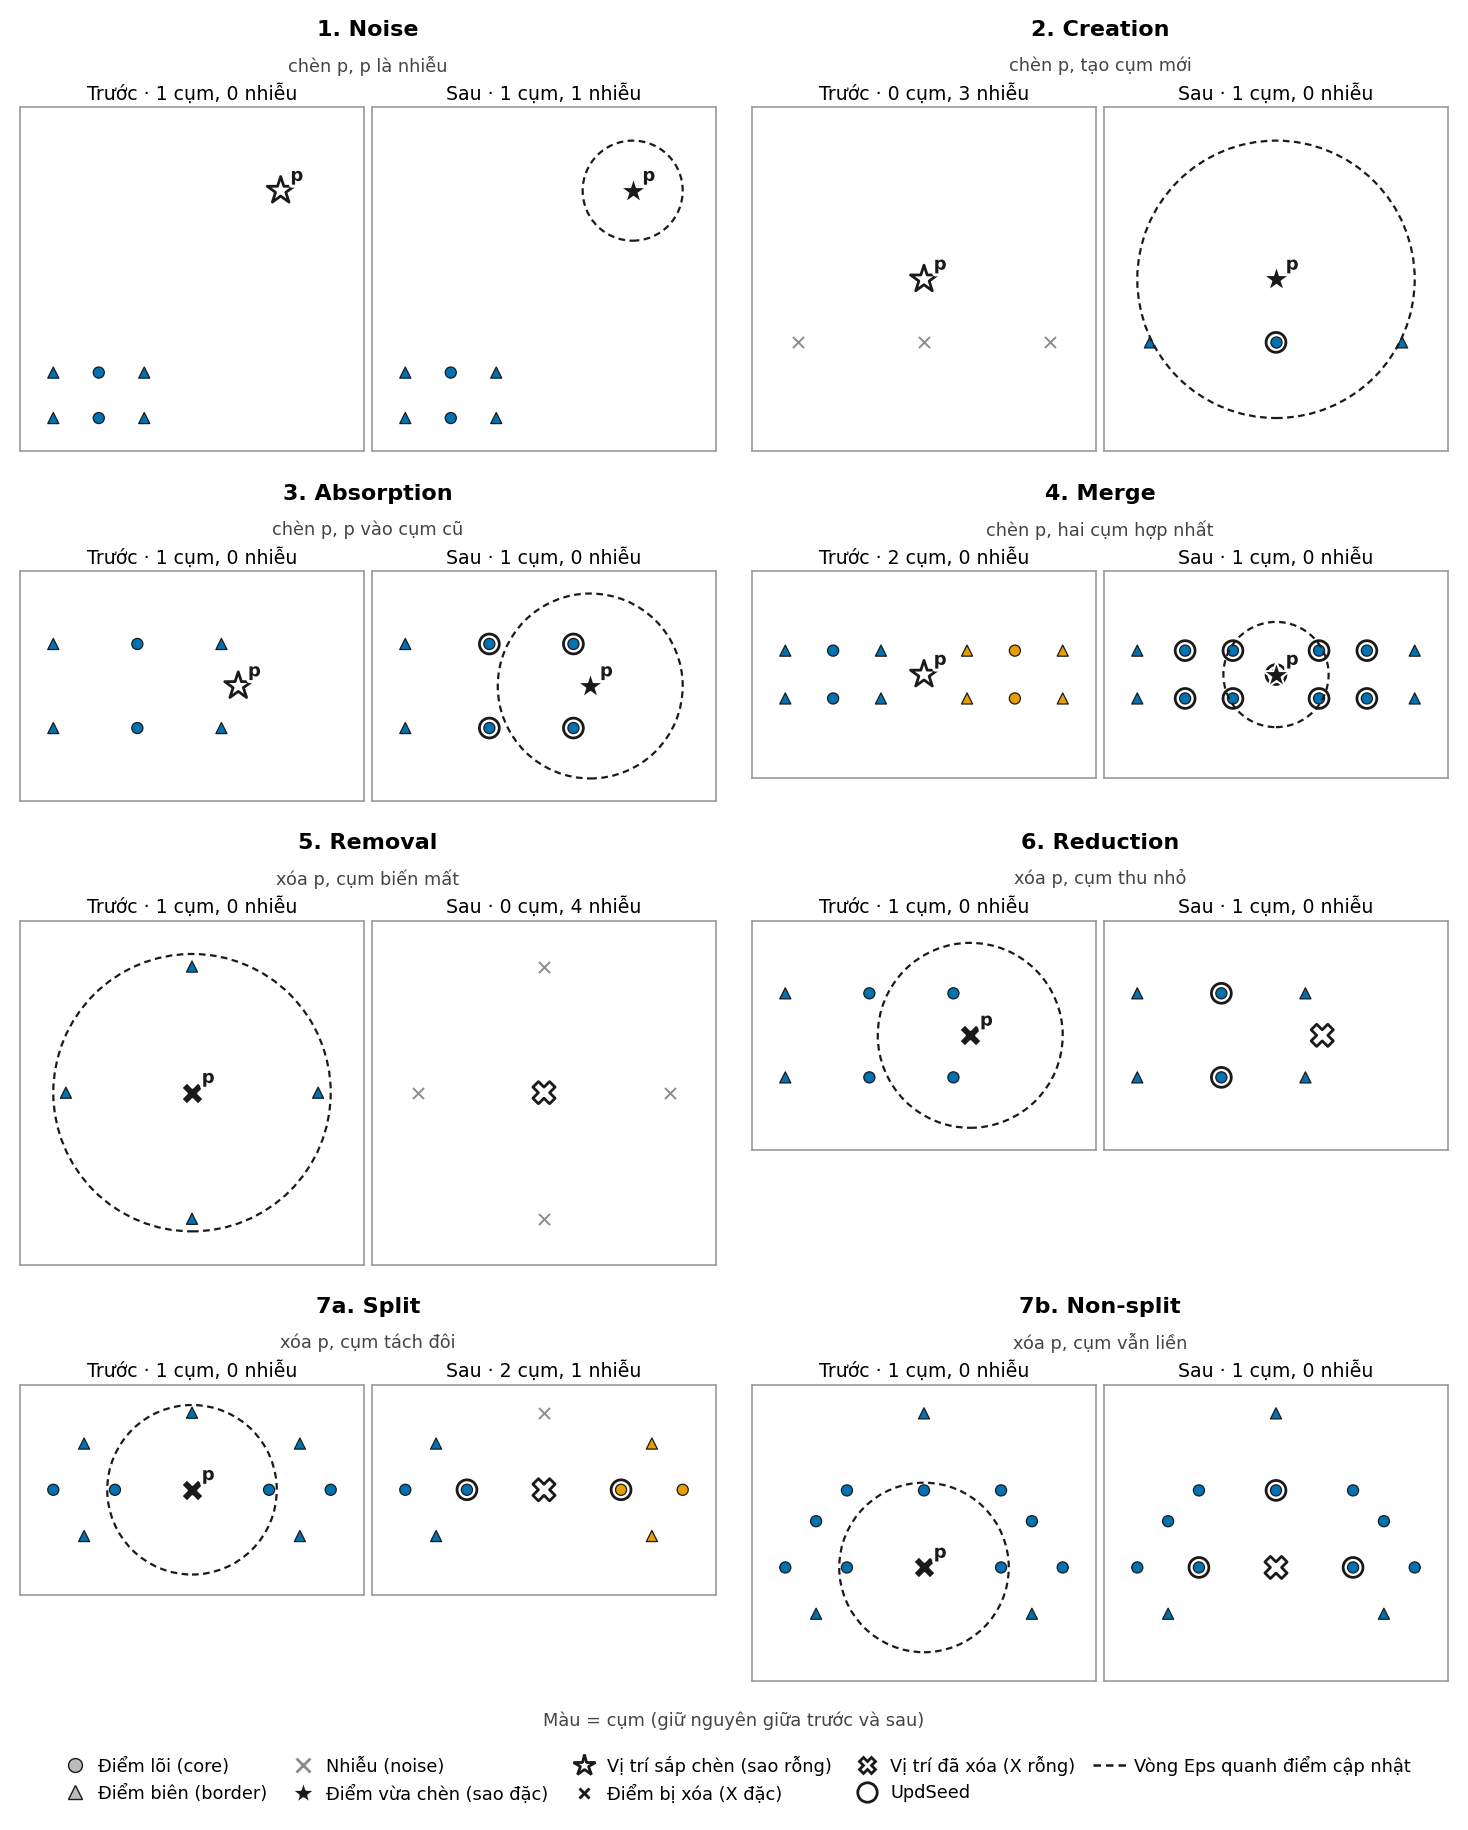
\includegraphics[
        width=\textwidth,
        trim=0bp 365bp 0bp 0bp,
        clip
    ]{Images/case_gallery_insert_delete.png}
    \caption{Minh họa các trường hợp cập nhật khi chèn đối tượng: Noise, Creation, Absorption và Merge}
    \label{fig:insert_cases}
\end{figure}

\textbf{Trường hợp 1 - Noise (Nhiễu)}

Trường hợp Noise xảy ra khi phép chèn không tạo ra lõi mới và đối tượng \(p\) không nằm trong lân cận của bất kỳ lõi nào đã tồn tại. Khi đó, \(p\) không đủ điều kiện để bắt đầu một cụm và cũng không thể gia nhập cụm cũ dưới dạng đối tượng biên.

Xét sáu đối tượng \(A=(0;0)\), \(B=(1;0)\), \(C=(2;0)\), \(D=(0;1)\), \(E=(1;1)\) và \(F=(2;1)\), với \(\varepsilon=1{,}1\) và \(\mathrm{MinPts}=4\).

Trước cập nhật, \(B\) và \(E\) là hai đối tượng lõi, các đối tượng còn lại là biên và toàn bộ sáu đối tượng thuộc cùng một cụm \(C_1\).

Chèn thêm đối tượng \(p=(5;5)\). Do khoảng cách từ \(p\) đến mọi đối tượng cũ đều lớn hơn \(\varepsilon\), ta có:

\begin{equation}
N_{\varepsilon}(p)=\{p\},
\qquad |N_{\varepsilon}(p)|=1<4.
\end{equation}

Không có đối tượng cũ nào tăng số lượng lân cận, nên \(\mathrm{NewCore}=\varnothing\). Đồng thời, \(p\) không nằm trong lân cận của lõi \(B\) hoặc \(E\).

Kết quả, \(p\) được xác định là nhiễu và cụm \(C_1\) không thay đổi.

Lưu ý: \(\mathrm{NewCore}=\varnothing\) chưa đủ để kết luận \(p\) là nhiễu. Nếu \(p\) nằm trong lân cận của một lõi cũ, nó vẫn có thể được bổ sung vào cụm dưới dạng đối tượng biên mà không làm xuất hiện lõi mới.

\textbf{Trường hợp 2 - Creation (Tạo cụm mới)}

Creation xảy ra khi phép chèn tạo ra một hoặc nhiều đối tượng lõi, nhưng những kết nối mới không dẫn đến bất kỳ cụm nào đã tồn tại trước cập nhật.

Xét ba đối tượng \(A=(0;0)\), \(B=(1;0)\) và \(C=(2;0)\), với \(\varepsilon=1{,}1\) và \(\mathrm{MinPts}=4\).

Trước khi chèn, số lượng đối tượng trong lân cận của \(A\), \(B\), \(C\) lần lượt là 2, 3 và 2. Vì không có đối tượng lõi, cả ba đều được xác định là nhiễu.

Chèn đối tượng \(p=(1;0{,}5)\). Khoảng cách từ \(p\) đến \(B\) bằng \(0{,}5\), trong khi khoảng cách đến \(A\) và \(C\) đều lớn hơn \(1{,}1\). Do đó:

\begin{equation}
    N_{\varepsilon}(p)=\{B,p\}.
\end{equation}

Đối tượng \(B\) có số lượng lân cận tăng từ 3 lên 4:

\begin{equation}
    |N_{\varepsilon}(B)|:3\longrightarrow4.
\end{equation}

Vì đạt ngưỡng \(\mathrm{MinPts}\), \(B\) chuyển từ nhiễu thành lõi. Khi đó:

\begin{equation}
    \mathrm{NewCore}=\{B\},
    \qquad
    \mathrm{UpdSeed}_{Ins}=\{B\}.
\end{equation}

Từ lõi \(B\), các đối tượng \(A\), \(C\) và \(p\) đều khả đạt trực tiếp theo mật độ. Vì trước đó chưa có cụm nào, thuật toán tạo cụm mới:

\begin{equation}
    C_1=\{A,B,C,p\}.
\end{equation}

Trong kết quả này, \(B\) là lõi, còn \(A\), \(C\) và \(p\) là biên. Phép chèn chỉ tạo ra một lõi mới nhưng đủ để hình thành cụm gồm bốn đối tượng.

\textbf{Trường hợp 3 - Absorption (Bổ sung vào cụm hiện có)}

Absorption xảy ra khi các kết nối được tạo thêm chỉ liên hệ với một cụm đã tồn tại. Cụm này được mở rộng mà không cần hợp nhất với cụm khác. Trường hợp này cũng có thể xảy ra khi phép chèn không tạo ra lõi mới, nhưng đối tượng được chèn nằm trong lân cận của một lõi đã tồn tại và được bổ sung vào cụm dưới dạng đối tượng biên.

Xét sáu đối tượng \(A=(0;0)\), \(B=(1;0)\), \(C=(0;1)\), \(D=(1;1)\), \(E=(2;0)\) và \(F=(2;1)\), với \(\varepsilon=1{,}1\) và \(\mathrm{MinPts}=4\).

Trước cập nhật, \(B\) và \(D\) là lõi, bốn đối tượng còn lại là biên. Toàn bộ dữ liệu thuộc cùng một cụm \(C_1\).

Chèn đối tượng \(p=(2{,}2;0{,}5)\). Đối tượng mới nằm trong lân cận của \(E\) và \(F\), làm số lượng lân cận của hai đối tượng này tăng từ 3 lên 4:

\begin{equation}
\begin{aligned}
    |N_{\varepsilon}(E)| &:3\longrightarrow4,\\
    |N_{\varepsilon}(F)| &:3\longrightarrow4.
\end{aligned}
\end{equation}

Do đó, \(E\) và \(F\) chuyển từ biên thành lõi. Trong khi đó, \(p\) có ba đối tượng trong lân cận là \(E\), \(F\) và chính nó, nên vẫn là biên.

Từ hai lõi mới, thuật toán xác định:

\begin{equation}
    \mathrm{NewCore}=\{E,F\},
\end{equation}

\begin{equation}
    \mathrm{UpdSeed}_{Ins}=\{B,D,E,F\}.
\end{equation}

Vì \(B\) và \(D\) đều thuộc \(C_1\) trước cập nhật, các kết nối mới không liên hệ với cụm thứ hai. Thuật toán giữ nhãn cụm hiện có và bổ sung \(p\):

\begin{equation}
    C_1'=\{A,B,C,D,E,F,p\}.
\end{equation}

Kết quả là số thành viên của cụm tăng từ sáu lên bảy. Đồng thời, hai đối tượng \(E\) và \(F\) thay đổi từ biên thành lõi, nhưng số lượng cụm vẫn là một.

\textbf{Trường hợp 4 - Merge (Hợp nhất cụm)}

Merge xảy ra khi các kết nối thông qua lõi mới liên hệ những đối tượng lõi thuộc ít nhất hai cụm khác nhau trước cập nhật. Khi đó, các cụm liên quan trở thành một cụm sau khi chèn.

Xét hai cụm ban đầu với \(\varepsilon=1{,}1\) và \(\mathrm{MinPts}=4\).

Cụm thứ nhất gồm sáu đối tượng:

\begin{equation}
\begin{aligned}
C_1=\{&
A_1=(-1;0),A_2=(0;0),A_3=(1;0),\\
&A_4=(-1;1),A_5=(0;1),A_6=(1;1)\}.
\end{aligned}
\end{equation}

Cụm thứ hai cũng gồm sáu đối tượng:

\begin{equation}
\begin{aligned}
C_2=\{&
B_1=(2{,}8;0),B_2=(3{,}8;0),B_3=(4{,}8;0),\\
&B_4=(2{,}8;1),B_5=(3{,}8;1),B_6=(4{,}8;1)\}.
\end{aligned}
\end{equation}

Trước cập nhật, \(A_2\), \(A_5\), \(B_2\) và \(B_5\) là các đối tượng lõi. Hai cụm chưa có kết nối theo mật độ.

Chèn đối tượng \(p=(1{,}9;0{,}5)\). Khoảng cách từ \(p\) đến các đối tượng \(A_3\), \(A_6\), \(B_1\), \(B_4\) đều bằng:

\begin{equation}
    \sqrt{0{,}9^2+0{,}5^2}
    =\sqrt{1{,}06}\approx1{,}03<1{,}1.
\end{equation}

Vì vậy:

\begin{equation}
N_{\varepsilon}(p)=\{p,A_3,A_6,B_1,B_4\}.
\end{equation}

Đối tượng \(p\) có năm phần tử trong lân cận nên trở thành lõi. Đồng thời, \(A_3\), \(A_6\), \(B_1\) và \(B_4\) đều tăng số lượng lân cận từ 3 lên 4, do đó cũng trở thành lõi.

Tập lõi mới gồm:

\begin{equation}
    \mathrm{NewCore}=\{p,A_3,A_6,B_1,B_4\}.
\end{equation}

Khi xác định các đối tượng lõi trong lân cận của \(\mathrm{NewCore}\), ta thu được:

\begin{equation}
\begin{aligned}
\mathrm{UpdSeed}_{Ins}=\{&
A_2,A_3,A_5,A_6,\\
&B_1,B_2,B_4,B_5,p\}.
\end{aligned}
\end{equation}

Tập này chứa các lõi thuộc cả \(C_1\) và \(C_2\). Đặc biệt, lõi \(p\) kết nối với những lõi mới ở hai phía, tạo ra đường kết nối mật độ giữa hai cụm.

Vì vậy, thuật toán hợp nhất \(C_1\), \(C_2\) và \(p\) thành một cụm gồm 13 đối tượng:

\begin{equation}
    C=C_1\cup C_2\cup\{p\}.
\end{equation}

Trong chương trình của nhóm, việc hợp nhất được thực hiện bằng cách giữ lại một nhãn cụm và cập nhật nhãn của các thành viên thuộc cụm còn lại. Thuật toán xác định những cụm cần hợp nhất dựa trên các kết nối mới giữa những đối tượng lõi, thay vì tính lại lân cận của toàn bộ 13 đối tượng. Tuy nhiên, chương trình vẫn cần duyệt các đối tượng đang lưu để cập nhật nhãn của những đối tượng thuộc cụm bị hợp nhất.

\subsection{Các trường hợp khi xóa điểm}

\textbf{Nguyên tắc cập nhật khi xóa}

Khi xóa một đối tượng \(p\), số lượng phần tử trong lân cận của những đối tượng còn lại chỉ có thể giảm hoặc giữ nguyên. Vì vậy, những đối tượng trước đó không phải lõi không thể trở thành lõi do phép xóa, ngược lại, một số đối tượng lõi có thể mất tính chất lõi.

Phép xóa không tạo thêm các kết nối theo mật độ. Tuy nhiên, việc mất một đối tượng lõi không nhất thiết khiến cụm bị tách, bởi các đối tượng còn lại vẫn có thể được liên kết thông qua những lõi khác.

Ba trường hợp chính khi xóa là Removal, Reduction và Potential Split. Riêng Potential Split cần phân biệt hai kết quả: Split và Non-split.

\begin{table}[H]
\centering
\caption{Các trường hợp cập nhật khi xóa đối tượng}
\label{tab:incremental_delete_cases}
\normalsize
\begin{tabularx}{\textwidth}{|P{2.8cm}|Y|Y|}
\hline
\textbf{Trường hợp} & \textbf{Đặc điểm} & \textbf{Kết quả} \\
\hline
Removal &
Tập UpdSeedDel rỗng, không có đối tượng lõi còn lại nằm trong lân cận của những đối tượng vừa mất tính chất lõi. &
Đối tượng bị xóa, một số đối tượng có thể trở thành nhiễu. Cụm có thể biến mất nếu không còn lõi.
\\
\hline
Reduction &
Các đối tượng thuộc UpdSeedDel đều khả đạt trực tiếp theo mật độ từ nhau sau phép xóa. &
Cụm vẫn được duy trì nhưng có thể giảm số thành viên hoặc thay đổi tính chất của một số đối tượng. \\
\hline
Potential Split &
Các đối tượng thuộc UpdSeedDel trước đó thuộc cùng một cụm nhưng không còn khả đạt trực tiếp theo mật độ từ nhau. &
Cần kiểm tra xem các đối tượng còn kết nối thông qua những lõi khác hay không, từ đó xác định Split hoặc Non-split. \\
\hline
\end{tabularx}
\end{table}

\textbf{Quy trình DELETE trong chương trình của nhóm}

Phương thức \texttt{delete()} cập nhật cụm quanh điểm bị xóa. Quy trình dưới đây theo các bước mà nhóm đã cài đặt:

\begin{enumerate}[label=\textbf{Bước \arabic*.}, leftmargin=*, itemsep=4pt]
    \item Tìm điểm \(p\) cần xóa và lưu thông tin lân cận, nhãn cụm, trạng thái lõi của các điểm liên quan.
    \item Xóa \(p\) và bỏ ID của nó khỏi danh sách lân cận của các điểm còn lại.
    \item Tìm các điểm lõi bị mất trạng thái lõi. Từ các điểm này, tạo tập \(\mathrm{UpdSeed}_{Del}\), gồm các điểm lõi còn lại cần kiểm tra.
    \item Xét từng cụm liên quan. Nếu không có seed thì đó là Removal. Nếu các seed kề trực tiếp với nhau thì đó là Reduction và cụm không cần tách.
    \item Nếu các seed không kề trực tiếp, dùng BFS để lần theo các điểm lõi. Nếu BFS nối được các seed thì cụm không tách (Non-split); nếu không, các phần lõi bị rời nhau được gán thành các cụm riêng (Split).
    \item Cập nhật nhãn của các điểm lõi thuộc cụm bị tách, rồi phân loại lại các điểm không lõi liên quan thành biên hoặc nhiễu.
\end{enumerate}

Các điểm biên không được dùng làm cầu nối giữa hai cụm. Vì vậy, chương trình xác định kết nối giữa các điểm lõi trước, rồi mới gán lại trạng thái và nhãn cho những điểm biên hoặc nhiễu bị ảnh hưởng.

Cách làm này cũng xử lý được trường hợp xóa một điểm biên hoặc xóa điểm mà không làm điểm lõi nào mất trạng thái lõi.

\begin{figure}[H]
    \centering
    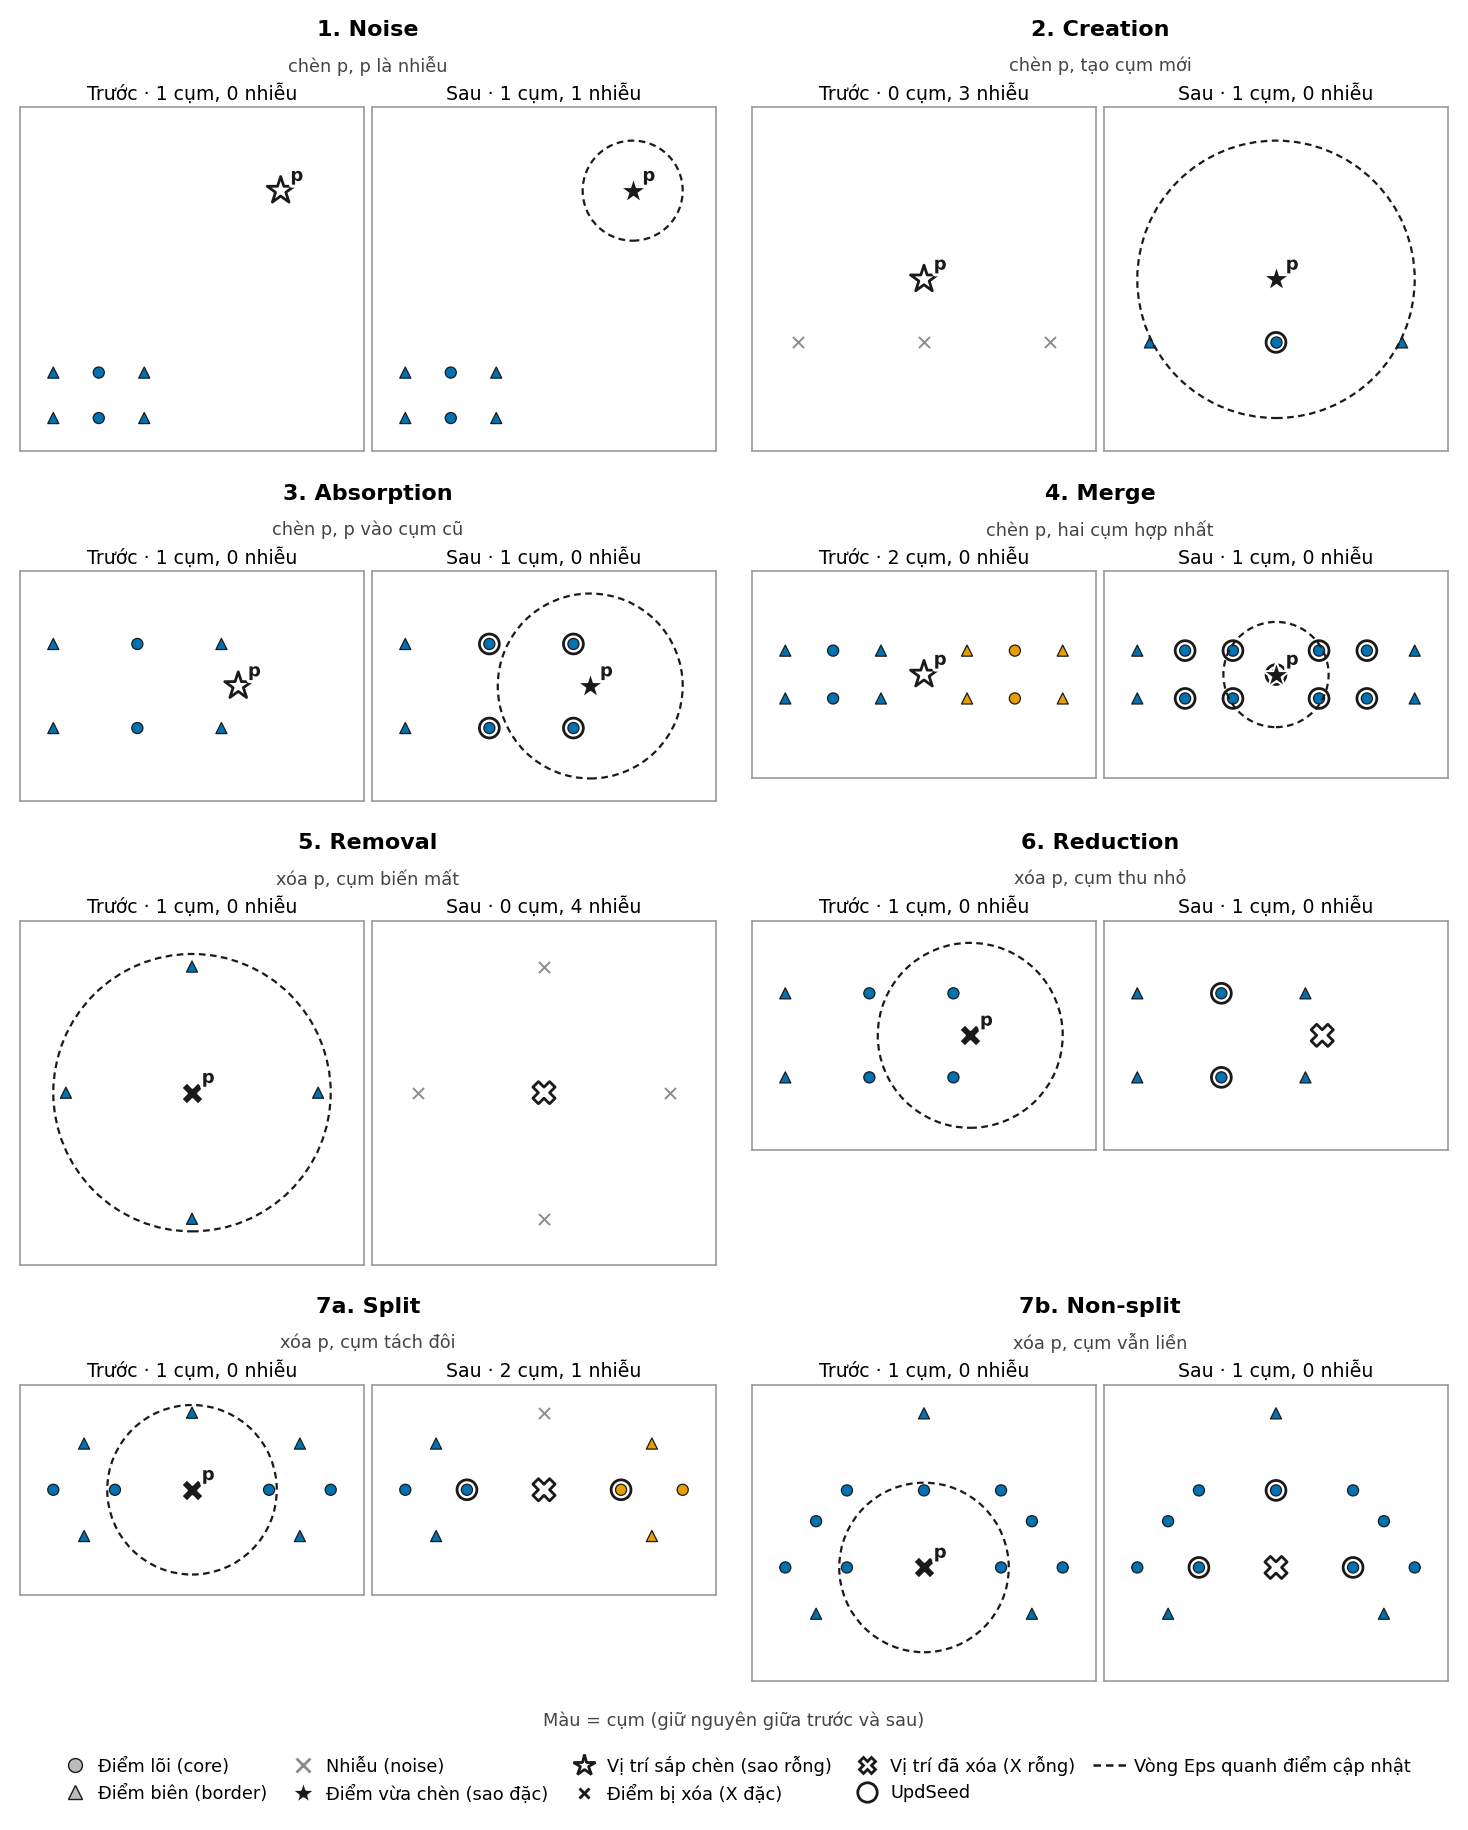
\includegraphics[
        width=\textwidth,
        trim=0bp 0bp 0bp 294bp,
        clip
    ]{Images/case_gallery_insert_delete.png}
    \caption{Minh họa các trường hợp cập nhật khi xóa đối tượng: Removal, Reduction, Split và Non-split}
    \label{fig:delete_cases}
\end{figure}

\textbf{Trường hợp 1 - Removal (Loại bỏ)}

Theo lý thuyết Incremental DBSCAN, Removal xảy ra khi tập UpdSeedDel rỗng, nghĩa là không còn đối tượng lõi nào trong lân cận của những đối tượng vừa mất tính chất lõi sau phép xóa. Khi đó, không cần tìm đường kết nối thay thế giữa các lõi. Nếu đối tượng bị xóa là lõi duy nhất duy trì một cụm, việc xóa có thể khiến cụm đó biến mất hoàn toàn.

Xét năm đối tượng:

\begin{equation}
\begin{aligned}
A&=(-1;0), & B&=(1;0),\\
C&=(0;-1), & D&=(0;1),\\
p&=(0;0).
\end{aligned}
\end{equation}

Với \(\varepsilon=1{,}1\) và \(\mathrm{MinPts}=4\), đối tượng \(p\) có lân cận:

\begin{equation}
N_{\varepsilon}(p)=\{A,B,C,D,p\}.
\end{equation}

Do có năm phần tử trong lân cận, \(p\) là lõi. Bốn đối tượng còn lại đều nằm trong lân cận của \(p\) nhưng không đủ điều kiện lõi, nên được xác định là biên. Tập dữ liệu ban đầu hình thành một cụm gồm năm đối tượng.

Sau khi xóa \(p\), các đối tượng \(A\), \(B\), \(C\), \(D\) không còn nằm trong lân cận của bất kỳ lõi nào. Mỗi đối tượng chỉ còn chính nó trong lân cận, vì khoảng cách giữa các đối tượng còn lại đều lớn hơn \(1{,}1\).

Khi đó, không còn đối tượng nào thỏa mãn điều kiện lõi, và:

\begin{equation}
    \mathrm{UpdSeed}_{Del}=\varnothing.
\end{equation}

Trong kết quả sau cập nhật, cụm ban đầu không còn tồn tại, bốn đối tượng còn lại đều trở thành nhiễu:

\begin{equation}
    {N}=\{A,B,C,D\}.
\end{equation}

Ví dụ cho thấy xóa một đối tượng không chỉ làm giảm số lượng thành viên của cụm. Nếu đối tượng đó là lõi duy nhất, phép xóa có thể loại bỏ toàn bộ cấu trúc cụm.

\textbf{Trường hợp 2 - Reduction (Thu hẹp cụm)}

Reduction xảy ra khi các đối tượng thuộc UpdSeedDel vẫn khả đạt trực tiếp theo mật độ từ nhau sau phép xóa. Điều này cho thấy những kết nối trực tiếp cần thiết giữa các đối tượng lõi liên quan vẫn được duy trì, nên không cần tìm kiếm đường kết nối thay thế. Một số đối tượng có thể mất tính chất lõi hoặc trở thành nhiễu, khiến cụm giảm số thành viên nhưng không bị tách thành các cụm riêng biệt.

Xét tập dữ liệu gồm:

\begin{equation}
\begin{aligned}
A&=(0;0), & B&=(1;0),\\
C&=(0;1), & D&=(1;1),\\
E&=(2;0), & F&=(2;1),\\
p&=(2{,}2;0{,}5).
\end{aligned}
\end{equation}

Với \(\varepsilon=1{,}1\) và \(\mathrm{MinPts}=4\), trước cập nhật, các đối tượng \(B\), \(D\), \(E\) và \(F\) là lõi. Toàn bộ bảy đối tượng thuộc cùng một cụm.

Khi xóa \(p\), số lượng lân cận của \(E\) và \(F\) giảm từ 4 xuống 3:

\begin{equation}
\begin{aligned}
    |N_{\varepsilon}(E)| &:4\longrightarrow3,\\
    |N_{\varepsilon}(F)| &:4\longrightarrow3.
\end{aligned}
\end{equation}

Vì vậy, \(E\) và \(F\) mất tính chất lõi, trong khi \(B\) và \(D\) vẫn là lõi. Hai đối tượng này cách nhau một đơn vị, nhỏ hơn \(\varepsilon\), nên vẫn khả đạt trực tiếp theo mật độ từ nhau.

Theo cách xác định trong paper:

\begin{equation}
    \mathrm{UpdSeed}_{Del}=\{B,D\}.
\end{equation}

Các đối tượng \(E\) và \(F\) vẫn nằm trong lân cận của lõi \(B\) hoặc \(D\), nên chuyển thành biên chứ không trở thành nhiễu.

Kết quả sau cập nhật là:

\begin{equation}
    C_1'=\{A,B,C,D,E,F\}.
\end{equation}

Cụm giảm từ bảy xuống sáu thành viên nhưng vẫn duy trì cấu trúc liên thông. Đây là trường hợp có sự thay đổi tính chất lõi nhưng không làm mất kết nối giữa những phần còn lại của cụm.

\textbf{Trường hợp 3 - Potential Split (Khả năng tách cụm)}

Potential Split xảy ra khi phép xóa làm mất những kết nối trực tiếp cần thiết giữa các đối tượng lõi. Tuy nhiên, việc mất kết nối trực tiếp chưa đủ để kết luận cụm bị tách, bởi vẫn có thể tồn tại đường kết nối thông qua những lõi khác.

Để xác định kết quả, cần kiểm tra các chuỗi kết nối giữa những đối tượng lõi còn lại. Có hai khả năng:

\begin{itemize}
    \item \textbf{Split:} Không còn đường kết nối lõi giữa một số phần của cụm, cụm ban đầu tách thành nhiều cụm.
    \item \textbf{Non-split:} Vẫn tồn tại đường kết nối lõi thay thế, cụm không bị tách.
\end{itemize}

\textbf{Trường hợp A - Split (Tách cụm)}

Xét mười đối tượng trong không gian hai chiều với \(\varepsilon=1{,}1\) và \(\mathrm{MinPts}=4\):

\begin{equation}
\begin{aligned}
A&=(1;0), & B&=(0{,}2;0),\\
C&=(0{,}6;0{,}6), & D&=(0{,}6;-0{,}6),\\
E&=(3;0), & F&=(3{,}8;0),\\
G&=(3{,}4;0{,}6), & H&=(3{,}4;-0{,}6),\\
I&=(2;1), & p&=(2;0).
\end{aligned}
\end{equation}

Trước khi xóa, \(A\), \(B\), \(E\), \(F\) và \(p\) là các đối tượng lõi. Trong đó, \(p\) nằm giữa hai vùng đối tượng và có lân cận:

\begin{equation}
    N_{\varepsilon}(p)=\{A,E,I,p\}.
\end{equation}

Do \(p\) là lõi, nó tạo ra kết nối mật độ giữa hai phía của cụm thông qua các đối tượng \(A\) và \(E\). Toàn bộ mười đối tượng ban đầu thuộc cùng một cụm.

Sau khi xóa \(p\), các đối tượng \(A\) và \(E\) vẫn là lõi với số lượng lân cận giảm từ 5 xuống 4. Tuy nhiên, khoảng cách giữa chúng là:

\begin{equation}
    d(A,E)=2>\varepsilon.
\end{equation}

Vì vậy, \(A\) và \(E\) không còn kết nối trực tiếp. Đồng thời, không tồn tại chuỗi đối tượng lõi thay thế nối hai phía sau khi loại bỏ \(p\).

Đối tượng \(I\) cũng không còn nằm trong lân cận của lõi nào và chuyển thành nhiễu.

Kết quả, cụm ban đầu tách thành hai cụm:

\begin{equation}
    C_1=\{A,B,C,D\},
\end{equation}

\begin{equation}
    C_2=\{E,F,G,H\},
\end{equation}

và tập nhiễu:

\begin{equation}
    N =\{I\}.
\end{equation}

Ví dụ cho thấy một đối tượng lõi có thể đóng vai trò nối hai phần của cùng một cụm. Khi đối tượng đó bị xóa và không còn chuỗi kết nối lõi thay thế, hai phần sẽ trở thành những cụm riêng biệt.

\textbf{Trường hợp B - Non-split (Không tách cụm)}

Sử dụng dữ liệu của trường hợp A và bổ sung ba đối tượng:

\begin{equation}
    J=(1;1),\qquad K=(3;1),\qquad L=(2;2).
\end{equation}

Các tham số \(\varepsilon=1{,}1\) và \(\mathrm{MinPts}=4\) được giữ nguyên. Trước cập nhật, toàn bộ 13 đối tượng thuộc cùng một cụm.

Sau khi xóa \(p\), đối tượng \(I\) vẫn là lõi vì lân cận còn bốn đối tượng là \(I\), \(J\), \(K\) và \(L\). Đồng thời, \(J\) và \(K\) cũng tiếp tục thỏa mãn điều kiện lõi.

Mặc dù kết nối trực tiếp thông qua \(p\) không còn, thuật toán xác định được chuỗi lõi thay thế:

\begin{equation}
    A\rightarrow J\rightarrow I\rightarrow K\rightarrow E.
\end{equation}

Khoảng cách giữa từng cặp đối tượng liên tiếp trong chuỗi đều bằng 1, không vượt quá \(\varepsilon\). Hơn nữa, tất cả đối tượng trong chuỗi đều là lõi sau cập nhật, nên các quan hệ khả đạt trực tiếp theo mật độ vẫn được duy trì dọc theo chuỗi.

Vì vậy, hai phía của cụm vẫn có quan hệ kết nối theo mật độ. Kết quả là 12 đối tượng còn lại tiếp tục thuộc cùng một cụm.

Hai ví dụ Split và Non-split cho thấy việc mất một đối tượng lõi không tự động dẫn đến tách cụm. Yếu tố quyết định là sau phép xóa có còn tồn tại đường kết nối thông qua những đối tượng lõi khác hay không.

Trong code, BFS bắt đầu từ các điểm trong \(\mathrm{UpdSeed}_{Del}\) và chỉ đi qua những điểm lõi còn kề nhau. Nếu đã tìm thấy đường nối giữa các seed thì chương trình dừng việc kiểm tra tách cụm. Nếu không tìm thấy đường nối, chương trình xác định các phần lõi bị tách và cập nhật nhãn của chúng. Như vậy, phần cài đặt có dùng \(\mathrm{UpdSeed}_{Del}\); BFS là bước kiểm tra kết nối sau khi tạo tập seed.

\subsection{Khác biệt giữa Incremental DBSCAN và chạy lại DBSCAN}

Incremental DBSCAN (cập nhật tăng dần)  và chạy lại DBSCAN đều nhằm xác định cấu trúc gom cụm phù hợp với tập dữ liệu sau thay đổi. Điểm khác nhau nằm ở lượng thông tin được sử dụng lại và phạm vi cần xử lý.

Đối với cách chạy lại DBSCAN, mỗi lần cập nhật được xem như một bài toán gom cụm mới. Thuật toán thực hiện lại việc xác định lân cận, tính chất lõi và mở rộng cụm trên tập dữ liệu hiện tại.

Trong khi đó, Incremental DBSCAN giữ lại thông tin về đối tượng, lân cận, loại đối tượng và nhãn cụm sau mỗi lần xử lý. Khi phát sinh phép chèn hoặc xóa, thuật toán cập nhật những thông tin có thay đổi và điều chỉnh các cụm liên quan.

\begin{table}[H]
\centering
\caption{So sánh cách cập nhật kết quả gom cụm}
\label{tab:incremental_vs_refit}
\normalsize
\begin{tabularx}{\textwidth}{|P{3.1cm}|Y|Y|}
\hline
\textbf{Tiêu chí} & \textbf{Chạy lại DBSCAN} & \textbf{Incremental DBSCAN của nhóm} \\
\hline
Thông tin ban đầu &
Gom cụm lại tập dữ liệu hiện tại. &
Sử dụng kết quả gom cụm và lân cận đã lưu. \\
\hline
Phép chèn &
Tính lại lân cận và mở rộng cụm trên toàn bộ dữ liệu. &
Cập nhật lân cận của điểm mới và những đối tượng liên quan, sau đó xử lý các kết nối mới. \\
\hline
Phép xóa &
Gom cụm lại toàn bộ dữ liệu còn lại. &
Xác định các cụm liên quan, kiểm tra lại các thành phần lõi và gán lại nhãn. \\
\hline
Bộ nhớ &
Phụ thuộc cách cài đặt và lưu trữ lân cận. &
Cần duy trì tập lân cận và trạng thái của từng đối tượng. \\
\hline
Chi phí cập nhật &
Phụ thuộc quy mô toàn bộ tập dữ liệu sau thay đổi. &
Phụ thuộc phạm vi các cụm liên quan, chi phí duy trì trạng thái và những thao tác duyệt dữ liệu cần thiết để cập nhật nhãn cụm.\\
\hline
\end{tabularx}
\end{table}

Nhờ lưu lại thông tin lân cận và trạng thái phân cụm, Incremental DBSCAN có thể hạn chế việc tính toán lại toàn bộ dữ liệu sau mỗi phép chèn hoặc xóa. Tuy nhiên, trong một số trường hợp như hợp nhất hoặc tách cụm, chương trình vẫn phải duyệt lại nhiều đối tượng để cập nhật nhãn và kiểm tra các kết nối còn lại.

Việc duy trì trạng thái cũng làm tăng nhu cầu lưu trữ so với những cách cài đặt không giữ lại toàn bộ thông tin lân cận. Vì vậy, Incremental DBSCAN không nhất thiết xử lý nhanh hơn DBSCAN chạy lại trong mọi tình huống. Lợi ích của phương pháp phụ thuộc vào phạm vi dữ liệu bị ảnh hưởng và lượng thông tin có thể tái sử dụng sau mỗi cập nhật.

\section{Các chỉ số đánh giá}

Nhóm xem kết quả theo ba khía cạnh: cập nhật có đúng không, các cụm có tách biệt không, và mất bao lâu để chạy. Silhouette là chỉ số chính để nhận xét chất lượng cụm; ARI chỉ giúp đối chiếu tính đúng đắn với DBSCAN chạy lại.

Nhóm cũng ghi nhận thời gian chạy, số cụm và tỷ lệ nhiễu để mô tả kết quả. Bộ nhớ được nhận xét qua lượng trạng thái thuật toán phải lưu; nhóm không đo bộ nhớ thành một thí nghiệm riêng.

\subsection{Adjusted Rand Index (ARI)}

Adjusted Rand Index (ARI) là chỉ số đo mức độ tương đồng giữa hai kết quả phân cụm trên cùng một tập dữ liệu. Chỉ số này dựa trên việc xem xét các cặp đối tượng có được xếp vào cùng nhóm hoặc khác nhóm trong cả hai kết quả hay không, đồng thời hiệu chỉnh mức độ tương đồng có thể xuất hiện do ngẫu nhiên.

Giá trị ARI được diễn giải như sau:

\begin{itemize}
    \item ARI = 1: Hai kết quả có cùng cách phân nhóm, không phụ thuộc vào giá trị số của nhãn cụm.
    \item ARI \(\approx 0\): Mức độ tương đồng xấp xỉ giá trị kỳ vọng khi phân nhóm ngẫu nhiên.
    \item ARI < 0: Mức độ tương đồng thấp hơn giá trị kỳ vọng nói trên.
\end{itemize}

Trong đồ án, ARI chỉ dùng để kiểm tra kết quả Incremental DBSCAN có gần với DBSCAN chạy lại trên cùng dữ liệu, khoảng cách và tham số hay không. Các điểm nhiễu vẫn được giữ lại; nhãn \(-1\) được xem là một nhãn riêng trong phép đối chiếu. ARI không phải chỉ số chính để đánh giá chất lượng cụm.

Tuy nhiên, ARI không phân biệt trực tiếp đối tượng lõi và đối tượng biên. Ngoài ra, một đối tượng biên có thể được gán hợp lệ vào nhiều cụm khác nhau. Vì vậy, nhóm còn kiểm tra riêng tính chất lõi, trạng thái nhiễu và các trường hợp gán cụm của đối tượng biên, thay vì chỉ dựa vào ARI.

\subsection{Silhouette}

Silhouette cho biết một điểm gần với cụm của nó đến mức nào và cách các cụm khác bao xa. Chỉ số này không cần nhãn đáp án có sẵn.

Với mỗi điểm \(i\), gọi \(a(i)\) là khoảng cách trung bình đến các điểm khác trong cùng cụm, còn \(b(i)\) là khoảng cách trung bình nhỏ nhất đến một cụm khác. Silhouette của điểm đó được tính như sau:

\begin{equation}
    s(i)=\frac{b(i)-a(i)}{\max\{a(i),b(i)\}}.
\end{equation}

Giá trị gần 1 thường có nghĩa điểm nằm gần cụm của mình và xa cụm khác; gần 0 là điểm nằm giữa các cụm; giá trị âm cho thấy điểm có thể gần cụm khác hơn cụm đang được gán.

Giá trị Silhouette nằm trong khoảng từ -1 đến 1, cụ thể như sau:

\begin{itemize}
    \item Gần 1: Đối tượng nằm gần các thành viên cùng cụm và tách biệt tương đối rõ với những cụm khác.
    \item Gần 0: Đối tượng có mức độ gần tương tự với cụm hiện tại và một cụm khác, cho thấy sự phân biệt giữa các cụm chưa rõ ràng.
    \item Gần -1: Đối tượng có xu hướng nằm gần một cụm khác hơn so với cụm hiện tại, có thể cho thấy việc gán cụm chưa phù hợp.
\end{itemize}

Silhouette của toàn bộ kết quả gom cụm được xác định bằng cách lấy trung bình giá trị Silhouette của các đối tượng được đưa vào đánh giá. Giá trị trung bình càng cao thường cho thấy các cụm càng tập trung và tách biệt rõ theo khoảng cách sử dụng.

\textbf{Cách nhóm tính Silhouette}

Nhóm tự cài phép tính Silhouette theo công thức trên. Các điểm nhiễu có nhãn \(-1\) được bỏ khỏi phép tính, còn các điểm thuộc cụm được giữ lại.

Chỉ tính điểm tổng hợp khi sau khi bỏ nhiễu còn ít nhất hai cụm. Nếu điều kiện này không đạt, kết quả được ghi là chưa xác định. Nếu một cụm chỉ có một điểm, Silhouette của điểm đó được quy ước bằng 0. Vì bỏ nhiễu có thể làm điểm trung bình tăng, nhóm đọc Silhouette cùng số cụm và tỷ lệ nhiễu.

\textbf{Giới hạn khi đánh giá DBSCAN bằng Silhouette}

Silhouette phản ánh sự gần nhau và tách biệt giữa các cụm dựa trên khoảng cách trung bình, nên thường thuận lợi cho những cụm có các đối tượng phân bố tập trung và cách xa nhau. Trong khi đó, DBSCAN có thể xác định những cụm có hình dạng không lồi. Với những dạng phân bố này, các đối tượng trong cùng cụm có thể cách nhau xa về mặt hình học nhưng vẫn được kết nối theo mật độ.

Vì vậy, Silhouette thấp không nhất thiết cho thấy DBSCAN gom cụm sai. Một kết quả phản ánh đúng các vùng kết nối theo mật độ vẫn có thể nhận Silhouette thấp hơn cách phân chia thành các cụm nhỏ, gọn hơn \parencite{sklearnClusteringGuide}.

Ngoài ra, khi loại nhiều đối tượng nhiễu khỏi phép tính, Silhouette trung bình có thể tăng do chỉ còn các đối tượng được gom vào những cụm rõ ràng hơn. Do đó, nhóm cần báo cáo Silhouette cùng số lượng hoặc tỷ lệ nhiễu để tránh đánh giá kết quả chỉ dựa trên những đối tượng được giữ lại.

\subsection{Thời gian chạy và bộ nhớ}

Thời gian thực hiện là một tiêu chí để đánh giá hiệu quả xử lý của Incremental DBSCAN. Khi so sánh với DBSCAN chạy lại, cần phân biệt thời gian gom cụm ban đầu và thời gian xử lý từng phép cập nhật. Chi phí cập nhật có thể thay đổi tùy theo loại thao tác và phạm vi cụm bị ảnh hưởng, do đó Incremental DBSCAN không nhất thiết nhanh hơn trong mọi trường hợp.

Bên cạnh thời gian xử lý, việc duy trì thông tin lân cận và trạng thái phân cụm cũng làm tăng nhu cầu bộ nhớ. Đây là sự đánh đổi giữa việc lưu trữ thông tin để tái sử dụng và việc phải tính toán lại từ đầu. Trong phạm vi đồ án, nhóm tập trung đo thời gian thực nghiệm, còn chi phí bộ nhớ được xem xét thông qua đặc điểm lưu trữ của thuật toán.

\subsection{Số cụm và số điểm nhiễu}

Số lượng cụm và số đối tượng nhiễu là những chỉ số mô tả trực tiếp kết quả gom cụm. Đối với Incremental DBSCAN, hai đại lượng này còn giúp theo dõi sự thay đổi cấu trúc dữ liệu sau mỗi phép chèn hoặc xóa.

Số cụm được xác định bằng cách đếm số nhãn cụm phân biệt trong kết quả, không tính nhãn -1 biểu thị nhiễu. Chẳng hạn, nếu tập dữ liệu có các nhãn {2, 2, 5, 5, -1}, kết quả gồm hai cụm và một đối tượng nhiễu. Số cụm được xác định dựa trên số nhãn phân biệt, không phụ thuộc vào giá trị cụ thể của các nhãn.

Số đối tượng nhiễu là số đối tượng mang nhãn -1 trong tập dữ liệu hiện tại. Tỷ lệ nhiễu cho biết tỷ lệ đối tượng không được gán vào cụm nào.

Đối với các phép cập nhật, nhóm theo dõi số cụm và số đối tượng nhiễu trước và sau thao tác để xác định những thay đổi trong kết quả gom cụm. Tuy nhiên, sự tăng hoặc giảm số cụm chưa đủ để xác định cụ thể trường hợp cập nhật đã xảy ra. Chẳng hạn, số cụm giảm có thể do hợp nhất hai cụm sau phép chèn hoặc do một cụm biến mất hoàn toàn sau phép xóa.

Tương tự, số đối tượng nhiễu tăng hoặc giảm có thể phản ánh sự thay đổi giữa trạng thái nhiễu và biên khi mật độ lân cận thay đổi. Vì vậy, nhóm kết hợp các đại lượng này với thông tin về loại đối tượng và quan hệ thành viên cụm để phân tích từng kịch bản.

Đối với các bộ dữ liệu mô phỏng có đối tượng nhiễu được xác định trước, số lượng và tỷ lệ nhiễu còn hỗ trợ đánh giá khả năng nhận diện các đối tượng nằm ngoài cấu trúc cụm.

\section{Các thuật toán dùng để so sánh}

Nhóm chọn DBSCAN, OPTICS và HDBSCAN để so sánh vì cả ba đều dựa trên mật độ nhưng tìm cụm theo những cách khác nhau. DBSCAN là đối chứng gần nhất với thuật toán nhóm tự cài. OPTICS và HDBSCAN giúp xem kết quả của hai cách phân cụm mật độ khác. Nhóm không đưa K-Means vào bảng so sánh chính vì K-Means thuộc cách phân cụm khác và không xử lý nhiễu như DBSCAN.

DBSCAN sử dụng hai tham số \(\varepsilon\) và \(\mathrm{MinPts}\) để xác định các đối tượng lõi và mở rộng cụm. OPTICS xây dựng thứ tự xử lý cùng khoảng cách khả đạt (Reachability Distance), qua đó hỗ trợ xem xét cấu trúc cụm ở nhiều ngưỡng mật độ. Trong khi đó, HDBSCAN xây dựng cấu trúc phân cấp dựa trên mật độ và lựa chọn những cụm có mức ổn định phù hợp, giúp nhận diện các cụm có mật độ khác nhau trong nhiều trường hợp \parencite{sklearnClusteringGuide}.

Trong benchmark, DBSCAN, HDBSCAN và OPTICS được lấy từ scikit-learn; sau mỗi cập nhật, các bản này được chạy lại trên toàn bộ dữ liệu hiện có. scikit-learn không cung cấp thao tác INSERT/DELETE tăng dần cho DBSCAN. Vì vậy, phép đo thời gian đối chiếu cập nhật cục bộ của chương trình nhóm với cách chạy lại toàn bộ, chứ không phải so sánh bốn thuật toán incremental.

Incremental DBSCAN vẫn dùng nguyên tắc mật độ của DBSCAN, nhưng tận dụng thông tin lân cận và cụm đã lưu để cập nhật sau INSERT hoặc DELETE.

Bảng~\ref{tab:clustering_algorithm_comparison} tổng hợp những đặc điểm chính của các thuật toán.

\begin{table}[H]
\centering
\caption{So sánh đặc điểm của các thuật toán gom cụm}
\label{tab:clustering_algorithm_comparison}
\normalsize
\begin{tabularx}{\textwidth}{|P{2.6cm}|Y|Y|}
\hline
\textbf{Thuật toán} &
\textbf{Nguyên tắc gom cụm} &
\textbf{Đặc điểm chính} \\
\hline
DBSCAN &
Kết nối các đối tượng theo mật độ với \(\varepsilon\) và \(\mathrm{MinPts}\). &
Nhận diện cụm không lồi và nhiễu; khó xử lý các cụm có mật độ chênh lệch lớn. \\
\hline

Incremental DBSCAN &
Tận dụng kết quả DBSCAN đã có để cập nhật cấu trúc cụm sau INSERT hoặc DELETE. &
Hỗ trợ chèn, xóa và sử dụng lại trạng thái, vẫn có thể cần duyệt nhiều đối tượng khi cập nhật nhãn cụm. \\
\hline

OPTICS &
Sắp xếp các đối tượng theo cấu trúc mật độ và khoảng cách khả đạt. &
Hỗ trợ phân tích cấu trúc cụm ở nhiều ngưỡng mật độ. \\
\hline

HDBSCAN &
Xây dựng và lựa chọn cụm từ cấu trúc phân cấp theo mật độ. &
Có thể nhận diện các cụm có mật độ khác nhau và xác định nhiễu. \\
\hline
\end{tabularx}
\end{table}

\chapter{TỔNG QUAN BỘ DỮ LIỆU}

\section{Nguồn gốc và cách sử dụng dữ liệu}

Các dữ liệu trong đề tài đều do nhóm mô phỏng bằng Python, không lấy từ khách hàng hay hệ thống ngân hàng thật. Nhóm dùng dữ liệu để minh họa DBSCAN trong không gian 2D, chạy các thao tác thêm/xóa và benchmark trên một luồng nhiều chiều.

Dữ liệu chính gồm tập tọa độ ATM 2D và luồng giao dịch thẻ 5D. Ngoài ra, nhóm chuẩn bị tám ví dụ nhỏ để minh họa các trường hợp cập nhật và một số ca nhỏ để kiểm thử tình huống biên.

\section{Mô tả các bộ dữ liệu}

\begin{table}[H]
\centering
\caption{Các bộ dữ liệu được dùng trong đề tài}
\label{tab:dataset_overview}
\normalsize
\begin{tabularx}{\textwidth}{@{}YP{4cm}P{2.5cm}@{}}
\toprule
\textbf{Bộ dữ liệu} & \textbf{Quy mô} & \textbf{Số chiều} \\
\midrule
ATM 2D & 1.200 điểm & 2 \\
Luồng thẻ & 500 điểm ban đầu, 300 cập nhật & 5 thuộc tính gốc \\
Ví dụ cập nhật & 8 kịch bản & 2 \\
Ca kiểm thử bổ sung & Một số ca nhỏ & 1D/2D \\
\bottomrule
\end{tabularx}
\end{table}

\textbf{ATM 2D.} Tập này có 1.200 điểm, mỗi điểm gồm hai tọa độ \texttt{x\_km} và \texttt{y\_km}. Các tọa độ mô phỏng vị trí trong mặt phẳng, đơn vị kilômét. Cột \texttt{point\_id} chỉ dùng để nhận diện điểm, không được đưa vào phép tính khoảng cách.

\textbf{Luồng giao dịch thẻ 5D.} Tập ban đầu \(D_0\) có 500 giao dịch. Mỗi giao dịch có năm thuộc tính số:

\begin{table}[H]
\centering
\caption{Các thuộc tính của luồng giao dịch thẻ}
\label{tab:card_features}
\normalsize
\begin{tabularx}{\textwidth}{@{}P{5cm}YP{1.7cm}@{}}
\toprule
\textbf{Thuộc tính} & \textbf{Ý nghĩa mô phỏng} & \textbf{Đơn vị} \\
\midrule
\texttt{amount\_vnd} & Giá trị giao dịch & VNĐ \\
\texttt{hour\_of\_day} & Giờ thực hiện giao dịch trong ngày & Giờ \\
\texttt{distance\_from\_home\_km} & Khoảng cách từ nơi giao dịch đến nhà & km \\
\texttt{txns\_last\_7d} & Số giao dịch trong bảy ngày trước đó & Lần \\
\texttt{merchant\_risk\_score} & Điểm rủi ro mô phỏng, từ 0 đến 1 & Điểm \\
\bottomrule
\end{tabularx}
\end{table}

Cột \texttt{point\_id} là mã định danh, không phải đặc trưng để gom cụm. Các giá trị được tạo để mô phỏng, nên không thể xem là mô tả hành vi của khách hàng ngoài đời.

\textbf{Các ví dụ cập nhật và ca kiểm thử bổ sung} 

Tám ví dụ nhỏ minh họa Noise, Creation, Absorption, Merge, Removal, Reduction, Split và Non-split. Mỗi ví dụ có dữ liệu ban đầu, một thao tác cập nhật và tệp \texttt{expected.json} ghi kết quả mong đợi. Một số test dùng tọa độ ngắn hoặc fixture riêng để kiểm tra tình huống biên; đây là các ca chức năng nhỏ, không phải bộ dữ liệu dùng để báo cáo benchmark.

\section{Tập ban đầu và các thao tác cập nhật}

Tập \(D_0\) được gom cụm trước bằng DBSCAN. Sau đó chương trình đọc lần lượt các dòng trong \texttt{updates.csv}: thao tác INSERT thêm một điểm, thao tác DELETE xóa một điểm đang có. File có tổng cộng 300 thao tác, gồm 150 INSERT và 150 DELETE xen kẽ; vì vậy số điểm trong luồng dao động từ 500 đến 501.

Thư mục \path{data/raw/card_stream/} chứa tập ban đầu, luồng cập nhật và file tham số. Trong \texttt{updates.csv}, cột \texttt{ambiguous\_border\_ids} là metadata tùy chọn cho bước đối chiếu các điểm biên; thuật toán không dùng cột này để quyết định cụm.

\section{Các chiều dữ liệu trong benchmark}

Benchmark 2D, 3D và 4D lấy các đặc trưng từ cùng luồng thẻ 5D, không phải ba bộ dữ liệu độc lập. Cấu hình 2D dùng số tiền đã lấy log và giờ giao dịch; 3D thêm khoảng cách từ nhà; 4D thêm số giao dịch trong bảy ngày. Điểm rủi ro của cửa hàng có trong dữ liệu gốc nhưng không dùng trong ba cấu hình này.

Các đặc trưng của thẻ được chuẩn hóa bằng những hằng số cố định lưu trong \texttt{params.json}, rồi dùng cùng dữ liệu đã chuyển đổi cho các thuật toán được so sánh. Hằng số được tính từ toàn bộ luồng mô phỏng để giữ cách biến đổi nhất quán giữa các lượt; đây là giới hạn của thí nghiệm, vì khi chạy online thực tế ta thường chưa biết các giao dịch trong tương lai.

Luồng có 300 cập nhật, nhưng benchmark thời gian giữa bốn thuật toán chạy trên 20 cập nhật đầu để giữ thời gian thực nghiệm vừa phải. Vì 2D, 3D và 4D dùng cùng các điểm và cùng thứ tự cập nhật, kết quả giữa các chiều cho biết việc thêm đặc trưng ảnh hưởng thế nào trong thí nghiệm này; không nên xem chúng như ba lần thử độc lập.

\section{Giới hạn của dữ liệu}

Các bộ dữ liệu chỉ là mô phỏng và có quy mô nhỏ, nên kết quả dùng để minh họa và kiểm tra cách thuật toán hoạt động. Chúng chưa đủ để kết luận thuật toán sẽ có hiệu quả tương tự trên dữ liệu ngân hàng thật hoặc ở quy mô lớn.

\chapter{TIỀN XỬ LÝ VÀ CÀI ĐẶT}

\section{Môi trường và thư viện sử dụng}

Chương trình được viết bằng Python và chia mã theo chức năng trong thư mục \texttt{src/}. Các phiên bản thư viện được khai báo trong \texttt{requirements.txt}. NumPy hỗ trợ thao tác với vector tọa độ, Pandas đọc và quản lý dữ liệu dạng bảng, còn Matplotlib được dùng để vẽ kết quả. Jupyter Notebook dùng để trình bày demo và benchmark.

DBSCAN và Incremental DBSCAN trong \texttt{src/clustering/} do nhóm tự cài đặt. Mã thuật toán không gọi hàm phân cụm của scikit-learn hay SciPy. scikit-learn chỉ được dùng trong phần đối chứng và đánh giá phụ; các hàm Silhouette chính của nhóm được cài riêng trong \texttt{src/evaluation/metrics.py}.

\begin{table}[H]
\centering
\caption{Thư viện và mục đích sử dụng}
\label{tab:environment_libraries}
\begin{tabularx}{\textwidth}{|P{3.2cm}|Y|}
\hline
\textbf{Thành phần} & \textbf{Mục đích trong đồ án} \\
\hline
Python & Cài đặt DBSCAN, Incremental DBSCAN, tiền xử lý và các bước thực nghiệm. \\
\hline
NumPy & Lưu và biến đổi vector số; hỗ trợ khoảng cách và phép chiếu dữ liệu khi vẽ. \\
\hline
Pandas & Đọc CSV và quản lý dữ liệu dạng bảng. \\
\hline
Matplotlib & Trực quan hóa cụm, điểm lõi, điểm biên và điểm nhiễu. \\
\hline
scikit-learn & Chạy DBSCAN, HDBSCAN và OPTICS làm đối chứng; không được gọi trong mã thuật toán tự cài. \\
\hline
Jupyter & Trình bày demo từng bước và notebook so sánh thuật toán. \\
\hline
\end{tabularx}
\end{table}

\section{Khảo sát dữ liệu}

Trước khi chạy thuật toán, nhóm kiểm tra tên cột, số dòng, mã điểm và thứ tự các thao tác. Kết quả kiểm tra các file chính được tóm tắt ở Bảng~\ref{tab:input_data_checks}. Chi tiết ý nghĩa thuộc tính đã trình bày trong Chương 3.

\begin{table}[H]
\centering
\caption{Kiểm tra ban đầu các file dữ liệu được dùng}
\label{tab:input_data_checks}
\begin{tabularx}{\textwidth}{|P{3.6cm}|P{2.5cm}|Y|}
\hline
\textbf{File} & \textbf{Số dòng} & \textbf{Kết quả kiểm tra} \\
\hline
\texttt{atm\_txn\_2d.csv} & 1.200 & Có hai cột tọa độ dùng để phân cụm; không thiếu giá trị ở các cột sử dụng và không lặp mã điểm. \\
\hline
\makecell[l]{\texttt{card\_stream/}\\\texttt{d0.csv}} & 500 & Có năm thuộc tính số; không thiếu giá trị ở các cột sử dụng và không lặp mã điểm ban đầu. \\
\hline
\makecell[l]{\texttt{card\_stream/}\\\texttt{updates.csv}} & 300 & Có 150 thao tác INSERT và 150 thao tác DELETE; số bước chạy liên tục từ 1 đến 300. \\
\hline
\end{tabularx}
\end{table}

Trong file cập nhật, các cột \texttt{step}, \texttt{op} và \texttt{point\_id} dùng để điều khiển luồng; chúng không phải đặc trưng khoảng cách. Ô trống ở \texttt{ambiguous\_border\_ids} là thông tin phụ tùy chọn, không phải giá trị của một đặc trưng được đưa vào mô hình.

\section{Làm sạch dữ liệu}

Các file dùng trong demo là dữ liệu mô phỏng có cấu trúc xác định. Nhóm giữ nguyên các dòng dữ liệu, không tự điền giá trị thiếu và không loại điểm chỉ vì điểm đó nằm xa các điểm khác; những điểm này có thể chính là nhiễu mà DBSCAN cần nhận diện. Các mã định danh được giữ riêng, không đưa vào vector đặc trưng.

Khi đọc dữ liệu để chuẩn hóa, \texttt{ManualScaler} kiểm tra số chiều và từ chối giá trị không phải số, NaN hoặc vô cùng. Nếu một cột có độ lệch chuẩn hoặc khoảng biến thiên bằng 0, chương trình dùng hệ số chia bằng 1 để tránh phép chia cho 0. Việc kiểm tra này giúp phát hiện dữ liệu đầu vào không hợp lệ trước khi tính khoảng cách.

\section{Chuẩn hóa dữ liệu}

Tọa độ ATM có đơn vị kilômét, nên nhóm giữ nguyên hai tọa độ \texttt{x\_km} và \texttt{y\_km}; tham số Eps của demo ATM cũng được tính theo kilômét. Với luồng giao dịch thẻ, các thuộc tính có đơn vị và thang đo khác nhau. Nhóm lấy log cơ số 10 của số tiền giao dịch, sau đó chuẩn hóa Z-score theo công thức:

\begin{equation}
    z_j = \frac{x_j - \mu_j}{\sigma_j},
\end{equation}

trong đó \(x_j\) là giá trị của thuộc tính, \(\mu_j\) là trung bình và \(\sigma_j\) là độ lệch chuẩn đã lưu trong \texttt{params.json}. Lớp \texttt{ManualScaler} tự tính và áp dụng phép biến đổi này, không dùng bộ chuẩn hóa của scikit-learn.

Các hằng số của luồng thẻ được giữ cố định khi xử lý D0 và các điểm cập nhật, để tọa độ của những điểm cũ không đổi sau mỗi thao tác. Chúng được tính từ toàn bộ luồng mô phỏng, kể cả các bước về sau; vì vậy cách làm phù hợp để so sánh có cùng đầu vào, nhưng chưa mô phỏng một hệ thống trực tuyến không biết dữ liệu tương lai.

\section{Thiết lập tập ban đầu và luồng cập nhật}

Với luồng thẻ, nhóm đọc 500 điểm trong \(D_0\), chọn đúng các cột đặc trưng của cấu hình, áp dụng phép biến đổi đã lưu rồi dùng DBSCAN để tạo trạng thái ban đầu. Chương trình tiếp tục đọc \texttt{updates.csv} theo cột \texttt{step}. Mỗi dòng INSERT thêm một điểm vào mô hình; mỗi dòng DELETE xóa điểm có mã tương ứng.

Benchmark so sánh bốn phương pháp trên cùng \(D_0\), tọa độ đã chuẩn hóa và thứ tự cập nhật. Nó chạy 20 thao tác đầu trong luồng 300 bước, gồm 10 INSERT và 10 DELETE. Incremental DBSCAN cập nhật trạng thái đã lưu; ba thuật toán scikit-learn được chạy lại trên toàn bộ tập hiện có sau mỗi thao tác. Cách tổ chức này giúp tách rõ khác biệt giữa cập nhật cục bộ và phân cụm lại.

\section{Lựa chọn tham số eps và MinPts}

Eps là bán kính xác định lân cận; MinPts là số điểm tối thiểu trong lân cận để một điểm trở thành điểm lõi. Lân cận có tính chính điểm đang xét. Các cấu hình trong đồ án khác nhau theo từng mục đích, như Bảng~\ref{tab:parameter_configs}.

\begin{table}[H]
\centering
\caption{Các cấu hình Eps và MinPts trong đồ án}
\label{tab:parameter_configs}
\begin{tabularx}{\textwidth}{|P{3.4cm}|P{3.6cm}|P{2.4cm}|Y|}
\hline
\textbf{Dữ liệu / mục đích} & \textbf{Eps} & \textbf{MinPts} & \textbf{Lý do sử dụng} \\
\hline
Ví dụ cập nhật 2D & 1,1 & 4 & Được chọn để tạo rõ các trường hợp Noise, Creation, Absorption, Merge, Removal, Reduction và Split. \\
\hline
ATM 2D & 0,5 km & 4 & Dùng với tọa độ tính bằng kilômét để minh họa các cụm trên mặt phẳng. \\
\hline
Luồng thẻ 2D/3D/4D & 0,4 sau chuẩn hóa & 6 & Lấy từ \texttt{params.json} và giữ nguyên giữa các thuật toán, số chiều và các lượt benchmark. \\
\hline
\end{tabularx}
\end{table}

Trên D0 của luồng thẻ, nhóm đã thử một lưới nhỏ các giá trị Eps và MinPts rồi xem Silhouette cùng số cụm và tỷ lệ nhiễu. Eps = 0,4 và MinPts = 6 cho kết quả ổn định trong các lát 2D, 3D và 4D của thí nghiệm; đây là cấu hình tham chiếu dễ giải thích, không phải tham số tối ưu cho mọi dữ liệu. Các cấu hình của ví dụ 2D, ATM và benchmark phục vụ những mục tiêu khác nhau nên không dùng để so trực tiếp giá trị Eps với nhau.

\section{Thiết kế hướng đối tượng và sơ đồ lớp}

Mỗi lớp giữ một phần trách nhiệm riêng. \texttt{DataPoint} lưu mã điểm, tọa độ, trạng thái và tập láng giềng. \texttt{DistanceMetric} tính khoảng cách Euclidean. \texttt{DBSCAN} tạo cụm ban đầu, còn \texttt{IncrementalDBSCAN} kế thừa lớp này và bổ sung thao tác thêm, xóa điểm. \texttt{IncrementalEngine} cung cấp ảnh chụp trạng thái để các notebook và bộ vẽ nhận cùng một dạng dữ liệu. \texttt{ManualScaler} xử lý chuẩn hóa, còn \texttt{ClusterVisualizer} vẽ kết quả.

\begin{figure}[H]
\centering
\begin{tikzpicture}[
  classbox/.style={draw,rectangle,align=left,text width=4.1cm,inner sep=5pt,font=\normalsize},
  relation/.style={thick},
  dependency/.style={thick,dashed,-{Latex}},
  inheritance/.style={thick,-{Triangle[open,length=2.5mm,width=2.5mm]}}
]
\node[classbox] (point) at (-5.05,2.25) {\textbf{DataPoint}\par\rule{3.9cm}{0.4pt}\par id, coords, cluster\_id\par point\_type, neighbor\_ids};
\node[classbox] (dbscan) at (0,2.25) {\textbf{DBSCAN}\par\rule{3.9cm}{0.4pt}\par fit(), get\_labels()\par region\_query(), expand\_cluster()};
\node[classbox] (metric) at (5.05,2.25) {\textbf{DistanceMetric}\par\rule{3.9cm}{0.4pt}\par euclidean(first, second)};
\node[classbox] (pointtype) at (-5.05,-0.65) {\textbf{PointType}\par\rule{3.9cm}{0.4pt}\par UNCLASSIFIED, CORE\par BORDER, NOISE};
\node[classbox] (incremental) at (0,-0.65) {\textbf{Incremental}\par\textbf{DBSCAN}\par\rule{3.9cm}{0.4pt}\par insert(point)\par delete(point\_id)};
\node[classbox] (scaler) at (5.05,-0.65) {\textbf{ManualScaler}\par\rule{3.9cm}{0.4pt}\par fit(), transform()\par inverse\_transform()};
\node[classbox] (engine) at (0,-3.55) {\textbf{IncrementalEngine}\par\rule{3.9cm}{0.4pt}\par snapshot()\par thống kê điểm và cụm};
\node[classbox] (visualizer) at (5.05,-3.55) {\textbf{ClusterVisualizer}\par\rule{3.9cm}{0.4pt}\par plot\_2d()\par plot\_before\_after()};
\draw[relation,-{Diamond[open,length=2.5mm,width=2.5mm]}] (point.east) -- (dbscan.west);
\draw[dependency] (dbscan.east) -- (metric.west);
\draw[dependency] (point.south) -- (pointtype.north);
\draw[inheritance] (incremental.north) -- (dbscan.south);
\draw[inheritance] (engine.north) -- (incremental.south);
\draw[dependency] (visualizer.west) -- (engine.east);
\end{tikzpicture}
\caption{Sơ đồ các lớp chính trong chương trình}
\label{fig:report_class_diagram}
\end{figure}

Trong hình, hình thoi rỗng biểu thị DBSCAN quản lý các đối tượng DataPoint; mũi tên tam giác rỗng biểu thị kế thừa; đường nét đứt biểu thị lớp dùng hoặc đọc thông tin của thành phần khác.

\begin{table}[H]
\centering
\caption{Trách nhiệm của các lớp và phần hỗ trợ}
\label{tab:class_responsibilities}
\begin{tabularx}{\textwidth}{|P{3.2cm}|Y|P{4.2cm}|}
\hline
\textbf{Thành phần} & \textbf{Trách nhiệm} & \textbf{Mã nguồn} \\
\hline
DataPoint, PointType & Lưu thông tin và trạng thái của mỗi điểm. & \path{src/core/data_point.py} \\
\hline
DistanceMetric & Tính khoảng cách Euclidean giữa hai vector cùng số chiều. & \path{src/core/distance.py} \\
\hline
ManualScaler & Fit, lưu và áp dụng tham số chuẩn hóa. & \path{src/preprocessing/scaler.py} \\
\hline
DBSCAN & Fit dữ liệu ban đầu, tìm lân cận và mở rộng cụm. & \path{src/clustering/dbscan.py} \\
\hline
Incremental DBSCAN & Cập nhật lân cận và nhãn cụm khi insert/delete. & \path{src/clustering/incremental_dbscan.py} \\
\hline
Incremental Engine & Trả snapshot và thống kê trạng thái để demo, đánh giá và vẽ. & \path{src/experiments/engine.py} \\
\hline
ClusterVisualizer & Vẽ cụm, loại điểm và trạng thái trước/sau cập nhật. & \path{src/visualization/plotter.py} \\
\hline
Hàm đánh giá & Tính Silhouette; được tổ chức thành module hàm, không phải một class riêng. & \path{src/evaluation/metrics.py} \\
\hline
\end{tabularx}
\end{table}

Sơ đồ thể hiện các lớp hiện có trong mã. Nhóm không tạo class riêng cho bộ đánh giá hay bộ điều phối thí nghiệm vì các thao tác đó hiện được thực hiện bằng module hàm và notebook; cách tổ chức này giữ thiết kế ở mức cần thiết cho đồ án.

\section{Cài đặt DBSCAN và Incremental DBSCAN}

DBSCAN tính các điểm trong vùng Eps của mỗi điểm bằng khoảng cách Euclidean. Vùng lân cận có tính cả điểm trung tâm. Nếu số điểm trong vùng đạt MinPts, điểm trung tâm là điểm lõi; thuật toán dùng ngăn xếp LIFO để mở rộng cụm qua các điểm lõi lân cận. Điểm được nối vào cụm nhưng không đủ MinPts được ghi nhận là điểm biên; điểm không được nối vào cụm nào là nhiễu.

Incremental DBSCAN kế thừa trạng thái do DBSCAN tạo và giữ cache lân cận theo mã điểm. Khi insert, chương trình cập nhật lân cận, tìm \(\mathrm{NewCore}\), rồi tạo \(\mathrm{UpdSeed}_{Ins}\) từ các lõi trong lân cận của những điểm vừa thành lõi. Phần cập nhật được giới hạn trong các lõi mới: chương trình duyệt chúng bằng stack LIFO và dùng nhãn của các lõi cũ trong tập seed để xác định tạo cụm, hấp thụ hay hợp nhất cụm. Nhờ đó, chương trình không chạy lại DBSCAN trên toàn bộ dữ liệu.

Khi delete, chương trình tìm \(\mathrm{LostCore}\), gồm điểm bị xóa nếu nó là lõi và các điểm kề vừa mất điều kiện lõi. Từ lân cận của các điểm này, chương trình lập \(\mathrm{UpdSeed}_{Del}\). Nếu tập seed rỗng thì xử lý Removal; nếu các seed trực tiếp nối nhau thì xử lý Reduction. Với Potential Split, BFS dùng hàng đợi FIFO khởi tạo từ các seed để tìm đường qua các lõi còn lại. Nếu các seed được nối với nhau thì cụm không tách; nếu không, các thành phần lõi được gán lại thành cụm riêng.

Các vector đầu vào không bị giới hạn ở hai tọa độ. Khoảng cách và truy vấn lân cận dùng toàn bộ số chiều của vector; 2D được dùng cho ví dụ dễ nhìn, còn các lát 2D, 3D và 4D của luồng thẻ được phân cụm theo toàn bộ đặc trưng trong cấu hình tương ứng.

\section{Cài đặt đánh giá và trực quan hóa}

Nhóm tự cài Silhouette trong \texttt{src/evaluation/metrics.py}. Với mỗi điểm không phải nhiễu, chương trình tính khoảng cách trung bình đến điểm cùng cụm và khoảng cách trung bình nhỏ nhất đến một cụm khác, sau đó lấy trung bình điểm Silhouette. Điểm nhiễu được bỏ khỏi phép tính; điểm ở cụm đơn lẻ nhận giá trị 0. Khi dữ liệu sau khi bỏ nhiễu còn ít hơn hai cụm, hàm báo không thể tính Silhouette thay vì trả một kết quả gây hiểu nhầm.

Phần đối chiếu gọi DBSCAN của scikit-learn để fit lại toàn bộ dữ liệu sau mỗi thao tác, rồi kiểm tra cách chia cụm và trạng thái điểm. Đây là phần tham khảo độc lập, không tham gia vào mã thuật toán tự cài. Các hình được vẽ bằng Matplotlib; dữ liệu nhiều chiều có thể được chiếu xuống mặt phẳng bằng PCA viết bằng NumPy để hiển thị, nhưng phép phân cụm vẫn chạy trên số chiều gốc.

Hai notebook được sắp theo mục đích: \texttt{Incremental\_DBSCAN\_Demo.ipynb} đi qua ví dụ INSERT/DELETE và demo ATM 2D; \texttt{So\_sanh\_thuat\_toan.ipynb} trình bày Silhouette và benchmark với DBSCAN, HDBSCAN, OPTICS. Cách chia này giúp người xem theo dõi thuật toán trước rồi mới xem phần so sánh.

\chapter{THỰC NGHIỆM VÀ ĐÁNH GIÁ}

\section{Thiết lập thực nghiệm}

Nhóm thực hiện ba loại kiểm tra: chạy các ví dụ nhỏ để quan sát từng bước INSERT/DELETE, đối chiếu kết quả với DBSCAN chạy lại, và đo chất lượng cụm cùng thời gian cập nhật trên luồng thẻ mô phỏng.

\begin{table}[H]
\centering
\caption{Các cấu hình chính trong thực nghiệm}
\label{tab:experiment_setup}
\normalsize
\begin{tabularx}{\textwidth}{@{}P{3.2cm}YP{3.5cm}@{}}
\toprule
\textbf{Thí nghiệm} & \textbf{Dữ liệu} & \textbf{Cấu hình} \\
\midrule
Ví dụ INSERT/DELETE & Các kịch bản 2D trong Chương 2 & Eps = 1,1; MinPts = 4 \\
Minh họa ATM & 1.200 tọa độ mô phỏng & Eps = 0,5 km; MinPts = 4 \\
So sánh trên luồng thẻ & D0 có 500 điểm; benchmark phát lại 20 cập nhật đầu & Eps = 0,4; MinPts = 6; 2D, 3D và 4D \\
\bottomrule
\end{tabularx}
\end{table}

DBSCAN và Incremental DBSCAN OOP là phần nhóm tự cài. DBSCAN, HDBSCAN và OPTICS của scikit-learn được dùng làm đối chứng \parencite{sklearnDBSCAN,sklearnHDBSCAN,sklearnOPTICS}. Trong benchmark luồng thẻ, bốn phương pháp nhận cùng dữ liệu đã chuẩn hóa, khoảng cách Euclidean và thứ tự cập nhật. Ba thuật toán thư viện được chạy lại trên toàn bộ dữ liệu hiện có sau mỗi cập nhật; bản Incremental DBSCAN xử lý INSERT/DELETE trên trạng thái đã lưu. Các tham số riêng của từng phương pháp được trình bày ở Chương 4, Bảng~\ref{tab:comparison_parameters}. Demo ATM 2D dùng tọa độ kilômét chưa chuẩn hóa và cấu hình riêng.

Benchmark thời gian chạy 5 lượt, có một lượt khởi động không tính vào kết quả. Mỗi lượt dùng cùng dữ liệu và cùng thứ tự 20 cập nhật, gồm 10 INSERT và 10 DELETE. Bảng thời gian báo trung vị và độ lệch chuẩn. Silhouette được tính trên trạng thái cuối của 20 cập nhật trong một lần chạy xác định, không phải trung bình của 5 lượt thời gian.

\section{Kết quả khi thêm điểm}

Các ví dụ INSERT dùng \(\mathrm{Eps}=1{,}1\), \(\mathrm{MinPts}=4\). Bốn trường hợp cho thấy một điểm mới có thể là nhiễu, tạo cụm mới, gia nhập cụm đang có hoặc làm các cụm nhập lại với nhau.

\begin{table}[H]
\centering
\caption{Kết quả các trường hợp INSERT}
\label{tab:insert_results}
\normalsize
\begin{tabularx}{\textwidth}{@{}P{2.4cm}YY@{}}
\toprule
\textbf{Trường hợp} & \textbf{Điều xảy ra} & \textbf{Kết quả sau cập nhật} \\
\midrule
Noise & Điểm mới không đủ lân cận và không nằm cạnh điểm lõi. & Điểm mới được đánh dấu nhiễu; cụm cũ giữ nguyên. \\
Creation & Điểm mới làm một số điểm đạt điều kiện lõi, nhưng chưa nối tới cụm cũ. & Các điểm liên quan tạo thành cụm mới. \\
Absorption & Điểm mới hoặc các điểm lân cận mới đạt điều kiện lõi trong vùng của một cụm cũ. & Cụm cũ được mở rộng; một số điểm nhiễu có thể thành điểm biên. \\
Merge & Các điểm lõi mới tạo đường nối giữa hai cụm cũ. & Các cụm có liên quan được gộp thành một cụm. \\
\bottomrule
\end{tabularx}
\end{table}

Trong ví dụ Merge, dữ liệu ban đầu có hai cụm. Điểm \(p\) được chèn vào giữa và làm các điểm ở hai phía trở thành lõi. Tập \(\mathrm{UpdSeed}_{Ins}\) chạm tới cả hai cụm, nên chương trình gộp chúng. Hình~\ref{fig:report_insert_merge} thể hiện các bước từ trước khi chèn đến sau khi cập nhật.

\begin{figure}[H]
    \centering
    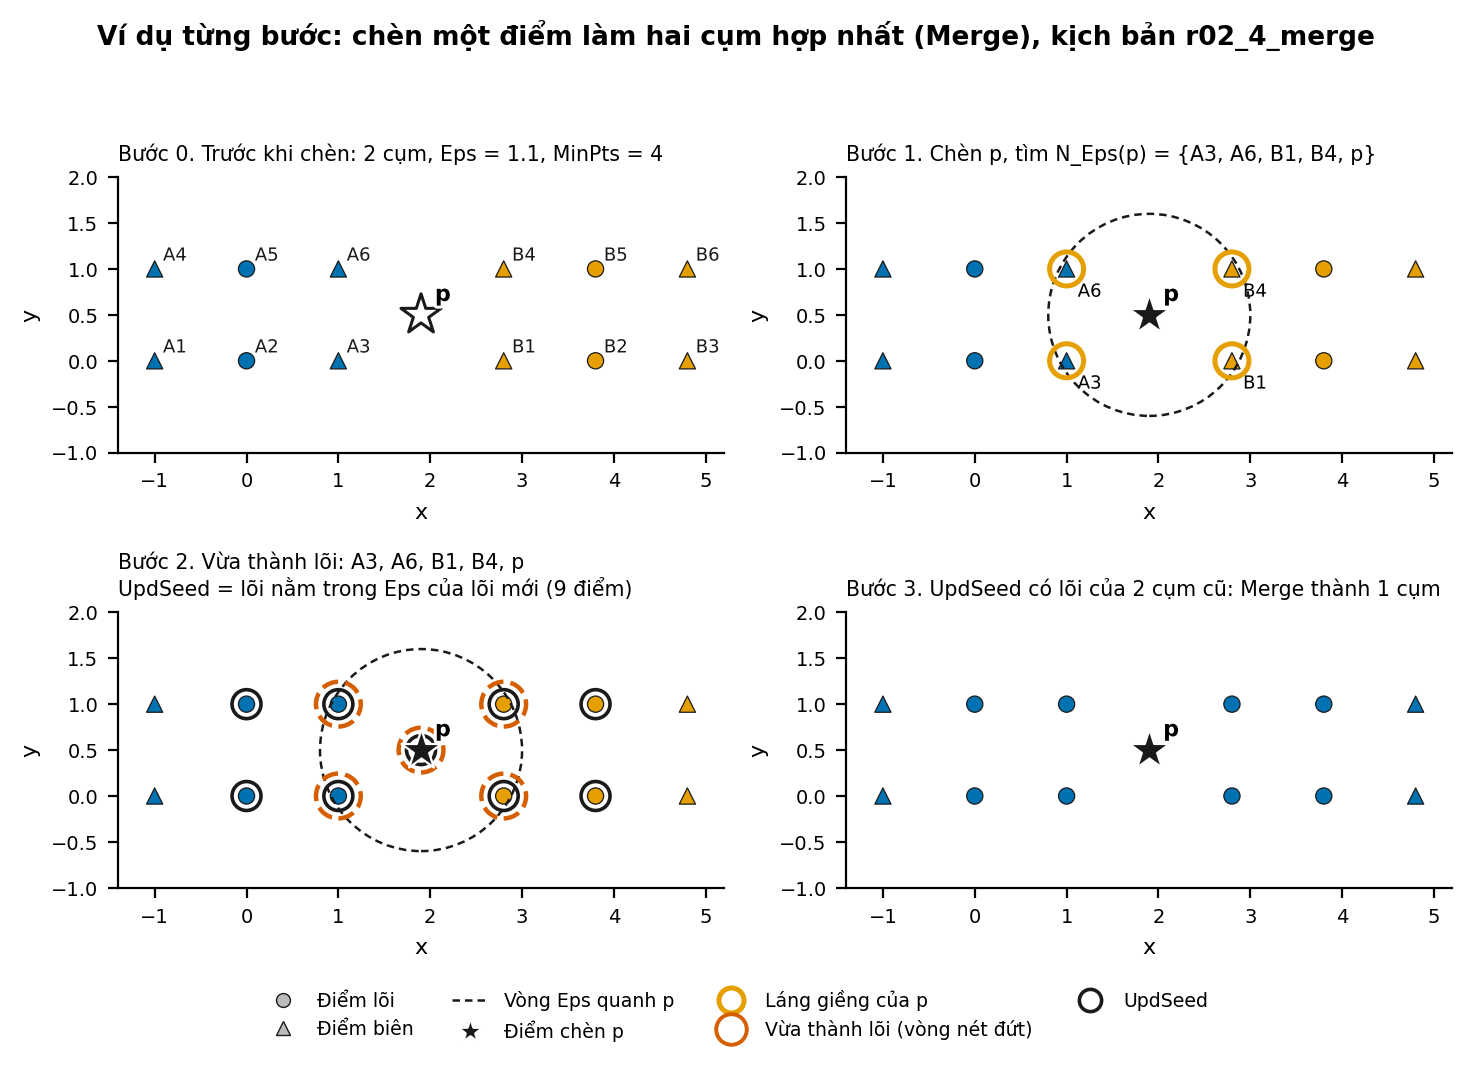
\includegraphics[width=0.98\textwidth]{Images/d05_steps_insert_merge.png}
    \caption{Các bước chèn điểm làm hai cụm nhập lại thành một cụm}
    \label{fig:report_insert_merge}
\end{figure}

\section{Kết quả khi xóa điểm}

Các ví dụ DELETE cũng dùng \(\mathrm{Eps}=1{,}1\), \(\mathrm{MinPts}=4\). Xóa một điểm không phải lúc nào cũng làm cụm bị tách. Kết quả phụ thuộc vào việc các điểm lõi còn giữ được đường nối hay không.

\begin{table}[H]
\centering
\caption{Kết quả các trường hợp DELETE}
\label{tab:delete_results}
\normalsize
\begin{tabularx}{\textwidth}{@{}P{2.8cm}YY@{}}
\toprule
\textbf{Trường hợp} & \textbf{Điều xảy ra} & \textbf{Kết quả sau cập nhật} \\
\midrule
Removal & Không còn seed lõi cần kiểm tra; có thể điểm bị xóa là lõi duy nhất của cụm. & Cụm có thể biến mất; các điểm còn lại thành nhiễu nếu không còn lõi nào. \\
Reduction & Các seed của cụm vẫn kề trực tiếp nhau. & Cụm không bị tách, dù một số điểm có thể mất trạng thái lõi và trở thành biên. \\
Potential Split - Split & BFS từ các seed không tìm được đường qua điểm lõi để nối các phía. & Cụm cũ tách thành nhiều cụm; điểm không còn cạnh lõi có thể thành nhiễu. \\
Potential Split - Non-split & Có đường nối thay thế qua các điểm lõi khác. & Cụm vẫn giữ nguyên, dù điểm cầu nối ban đầu đã bị xóa. \\
\bottomrule
\end{tabularx}
\end{table}

Ví dụ Split bắt đầu với một cụm có điểm \(p\) nối hai phía. Sau khi xóa \(p\), BFS không tìm được đường qua các điểm lõi giữa hai phía, nên cụm tách làm hai và điểm \(I\) trở thành nhiễu. Hình~\ref{fig:report_delete_split} minh họa kết quả này.

\begin{figure}[H]
    \centering
    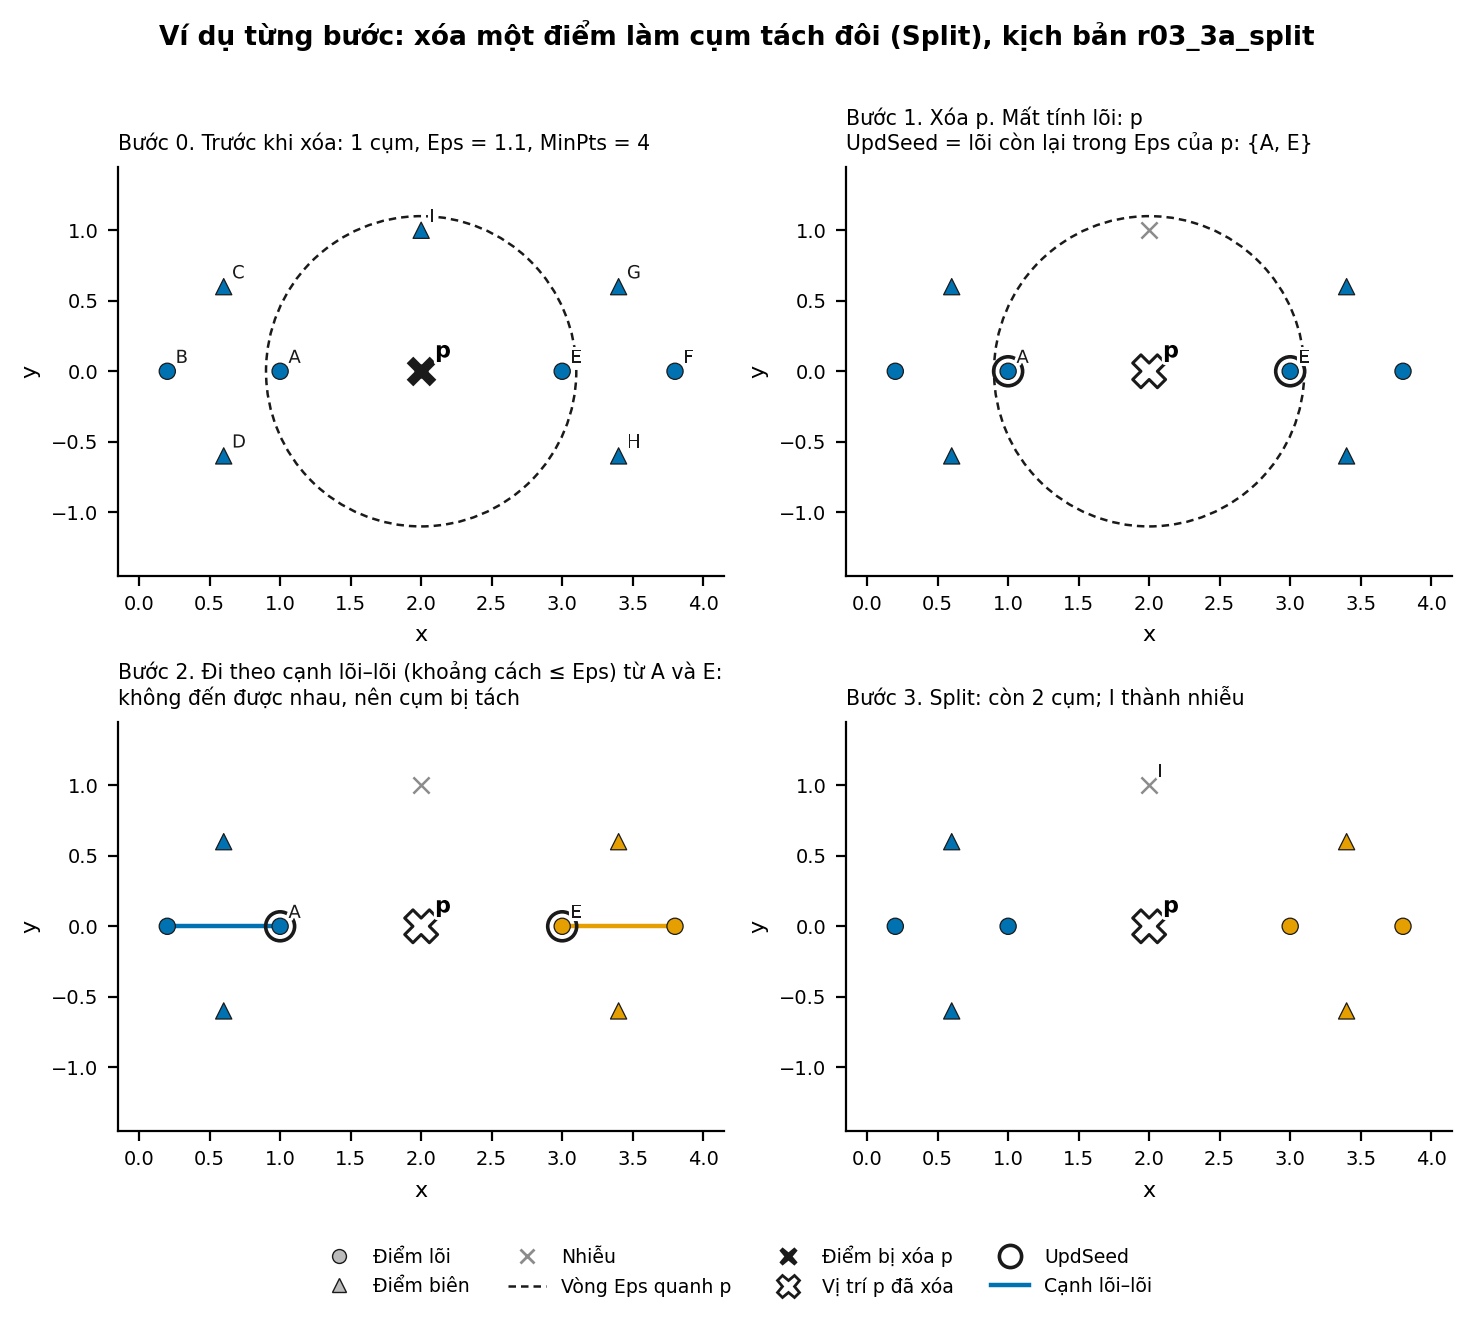
\includegraphics[width=0.98\textwidth]{Images/d06_steps_delete_split.png}
    \caption{Các bước xóa điểm cầu nối làm một cụm tách thành hai cụm}
    \label{fig:report_delete_split}
\end{figure}

Ở trường hợp Non-split, sau khi xóa điểm cầu nối ban đầu vẫn còn một đường đi qua các điểm lõi. Vì vậy BFS xác nhận các seed vẫn thuộc cùng một thành phần và không tách cụm. Hai trường hợp này cho thấy chỉ biết một điểm lõi bị xóa là chưa đủ; cần kiểm tra các đường nối còn lại.

\section{Minh họa trên không gian 2D}

Các ví dụ Merge và Split ở trên dùng tọa độ 2D để có thể theo dõi trực tiếp điểm mới, điểm bị xóa, vòng Eps và các điểm trong \(\mathrm{UpdSeed}\). Notebook minh họa trình bày từng bước của hai ví dụ này, sau đó chạy DBSCAN trên 1.200 tọa độ ATM.

Với ATM 2D, cấu hình Eps = 0,5 km và MinPts = 4 tạo ra 6 cụm, 142 điểm nhiễu; Silhouette tự cài trên các điểm không nhiễu là 0,3362. Các phương pháp nhận cùng hai tọa độ và khoảng cách Euclidean. DBSCAN dùng \texttt{eps=0.5, min\_samples=4}; HDBSCAN dùng \texttt{min\_cluster\_size=4, min\_samples=4} vì thuật toán này không có Eps; OPTICS dùng \texttt{min\_samples=4, eps=0.5, max\_eps=0.500001} và trích cụm theo kiểu DBSCAN. Vì Silhouette bỏ điểm nhiễu, nhóm đọc chỉ số này cùng số cụm và tỷ lệ nhiễu, không dùng riêng nó để kết luận mô hình nào tốt hơn.

\section{Đối chiếu với DBSCAN chạy lại}

Để kiểm tra phép cập nhật, nhóm so sánh trạng thái của Incremental DBSCAN với DBSCAN của scikit-learn được fit lại trên cùng tập điểm sau mỗi thao tác. Phép đối chiếu xét phân hoạch cụm, trạng thái lõi và điểm nhiễu; mã nhãn cụm có thể khác nhau nhưng cách chia điểm phải tương ứng.

Trong kết quả lưu tại \texttt{results/equivalence\_results.csv}, có 317 lần đối chiếu: 9 lần fit ban đầu, 154 INSERT và 154 DELETE. Cả 317 lần đều đạt điều kiện tương đương; không có trường hợp sai khác được ghi nhận. Kết quả này gồm các ví dụ cập nhật và luồng thẻ, cho thấy các trạng thái đã kiểm tra của bản OOP khớp với DBSCAN chạy lại.

Đây là kiểm tra trên các bộ dữ liệu và thao tác hiện có, không chứng minh thuật toán đúng với mọi dữ liệu có thể gặp.

\section{So sánh chất lượng cụm bằng Silhouette}

Nhóm tự cài Silhouette và dùng chỉ số này làm cách đánh giá chất lượng cụm chính. Điểm nhiễu bị bỏ khỏi phép tính, nên bảng luôn kèm số cụm và tỷ lệ nhiễu. ARI được dùng riêng để kiểm tra mức độ đồng thuận giữa hai cách cài DBSCAN, không dùng để xếp hạng HDBSCAN hay OPTICS.

Trên ATM 2D, các phương pháp cho kết quả sau:

\begin{table}[H]
\centering
\caption{So sánh Silhouette trên dữ liệu ATM 2D}
\label{tab:atm_silhouette}
\normalsize
\begin{tabularx}{\textwidth}{@{}Yccc@{}}
\toprule
\textbf{Phương pháp} & \textbf{Silhouette} & \textbf{Số cụm} & \textbf{Tỷ lệ nhiễu} \\
\midrule
Incremental DBSCAN OOP & 0,3362 & 6 & 11,83\% \\
scikit-learn DBSCAN & 0,3362 & 6 & 11,83\% \\
scikit-learn HDBSCAN & 0,3978 & 23 & 9,92\% \\
scikit-learn OPTICS & 0,3362 & 6 & 11,83\% \\
\bottomrule
\end{tabularx}
\end{table}

HDBSCAN có Silhouette cao hơn trong cấu hình này nhưng đồng thời tạo ra 23 cụm, nhiều hơn đáng kể so với sáu cụm của các phương pháp còn lại. Vì vậy, không thể chỉ nhìn điểm Silhouette rồi kết luận HDBSCAN tốt hơn; cần xem số cụm, tỷ lệ nhiễu và mục tiêu của bài toán.

Trên luồng thẻ, bảng dưới tính tại trạng thái cuối sau 20 cập nhật. Cả bốn phương pháp cho cùng 3 cụm và 1\% điểm nhiễu trong ba lát đặc trưng đang thử.

\begin{table}[H]
\centering
\caption{Silhouette trên các lát 2D, 3D và 4D của luồng thẻ}
\label{tab:card_silhouette}
\normalsize
\begin{tabularx}{\textwidth}{@{}ccccY@{}}
\toprule
\textbf{Số chiều} & \textbf{Silhouette} & \textbf{Số cụm} & \textbf{Nhiễu} & \textbf{Ghi chú} \\
\midrule
2D & 0,7785 & 3 & 1\% & Bốn phương pháp cho cùng phân hoạch trong cấu hình này. \\
3D & 0,7839 & 3 & 1\% & Bốn phương pháp cho cùng phân hoạch trong cấu hình này. \\
4D & 0,7463 & 3 & 1\% & Bốn phương pháp cho cùng phân hoạch trong cấu hình này. \\
\bottomrule
\end{tabularx}
\end{table}

Các lát 2D, 3D và 4D được lấy từ cùng một luồng dữ liệu, nên không phải ba bộ dữ liệu độc lập. Kết quả giống nhau giữa bốn phương pháp chỉ áp dụng cho dữ liệu, tham số và 20 cập nhật này; không có nghĩa các thuật toán luôn cho cùng kết quả.

\section{Thời gian chạy và giới hạn đo đạc}

Bảng~\ref{tab:update_runtime} báo tổng thời gian của 20 cập nhật, lấy trung vị \(\pm\) độ lệch chuẩn qua 5 lượt. Đơn vị là mili giây.

\begin{table}[H]
\centering
\caption{Thời gian cập nhật trên 20 thao tác}
\label{tab:update_runtime}
\normalsize
\begin{tabularx}{\textwidth}{@{}cYYYY@{}}
\toprule
\textbf{Dữ liệu} & \textbf{Incremental OOP} & \textbf{sklearn DBSCAN} & \textbf{sklearn HDBSCAN} & \textbf{sklearn OPTICS} \\
\midrule
Thẻ 2D & 321,08 \(\pm\) 25,53 & 136,72 \(\pm\) 14,81 & 198,41 \(\pm\) 18,84 & 14.571,56 \(\pm\) 238,01 \\
Thẻ 3D & 288,78 \(\pm\) 20,95 & 148,09 \(\pm\) 6,57 & 194,18 \(\pm\) 19,08 & 13.824,08 \(\pm\) 373,53 \\
Thẻ 4D & 194,56 \(\pm\) 9,98 & 152,03 \(\pm\) 8,23 & 208,37 \(\pm\) 22,12 & 13.485,85 \(\pm\) 232,03 \\
\bottomrule
\end{tabularx}
\end{table}

Trong phép đo này, DBSCAN scikit-learn fit lại có tổng thời gian thấp hơn bản OOP ở cả ba số chiều. HDBSCAN cũng nhanh hơn ở 2D và 3D, còn bản OOP thấp hơn một chút ở 4D. OPTICS có thời gian cao nhất trong cả ba cấu hình. Kết quả này không cho thấy Incremental DBSCAN luôn nhanh hơn cách fit lại; hình~\ref{fig:runtime_benchmark} thể hiện chênh lệch trên thang log.

\begin{figure}[H]
    \centering
    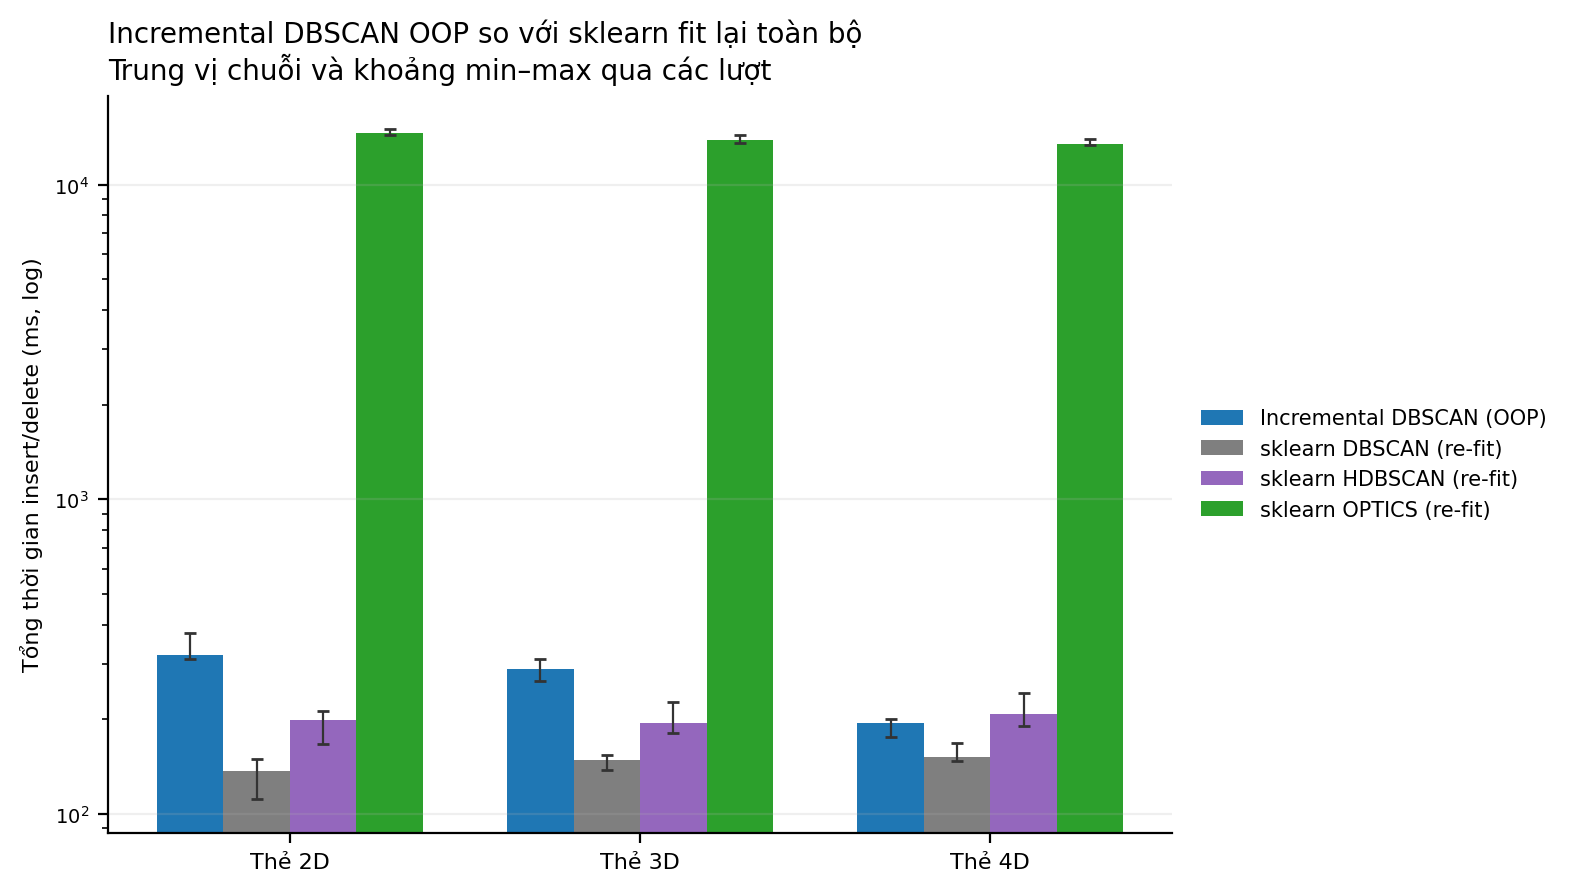
\includegraphics[width=0.9\textwidth]{Images/density_algorithm_benchmark.png}
    \caption{Tổng thời gian cập nhật qua 5 lượt benchmark}
    \label{fig:runtime_benchmark}
\end{figure}

Tuy vậy, thời gian fit ban đầu D0 của bản OOP cao hơn DBSCAN scikit-learn. Bảng~\ref{tab:initial_fit_runtime} tách riêng bước này để tránh chỉ nhìn thời gian cập nhật rồi kết luận bản OOP nhanh hơn trong toàn bộ quá trình.

\begin{table}[H]
\centering
\caption{Thời gian fit ban đầu D0, trung vị qua 5 lượt (ms)}
\label{tab:initial_fit_runtime}
\normalsize
\begin{tabularx}{\textwidth}{@{}cYYYY@{}}
\toprule
\textbf{Dữ liệu} & \textbf{Incremental OOP} & \textbf{sklearn DBSCAN} & \textbf{sklearn HDBSCAN} & \textbf{sklearn OPTICS} \\
\midrule
Thẻ 2D & 1.315,57 & 8,22 & 10,53 & 697,82 \\
Thẻ 3D & 1.288,58 & 7,75 & 10,46 & 701,88 \\
Thẻ 4D & 1.434,08 & 9,42 & 13,32 & 693,52 \\
\bottomrule
\end{tabularx}
\end{table}

Nhóm không đo bộ nhớ thành một thí nghiệm riêng. Phần này chỉ nhận xét định tính rằng Incremental DBSCAN phải lưu thêm lân cận và trạng thái điểm để dùng lại khi cập nhật. Thời gian nêu trên cũng chỉ phản ánh môi trường chạy, dữ liệu mô phỏng và 20 cập nhật đầu; không đại diện cho toàn bộ 300 cập nhật hay dữ liệu giao dịch thật.

\section{Nhận xét chung}

Các ví dụ nhỏ giúp quan sát rõ việc thêm điểm có thể tạo hoặc gộp cụm, còn xóa điểm có thể làm cụm giảm, biến mất hoặc tách ra. Kết quả đối chiếu hiện có không ghi nhận sai khác giữa Incremental DBSCAN và DBSCAN chạy lại. Trong benchmark thẻ, DBSCAN scikit-learn fit lại nhanh hơn bản OOP ở cả ba số chiều; HDBSCAN nhanh hơn ở 2D/3D và chậm hơn một chút ở 4D. Bước fit ban đầu của bản OOP cũng chậm hơn các phương pháp thư viện. Vì vậy, thí nghiệm hiện tại xác nhận tính đúng của cập nhật, nhưng chưa cho thấy lợi thế thời gian của bản OOP trên prefix 20 thao tác này.
\chapter{KẾT LUẬN VÀ HƯỚNG PHÁT TRIỂN}

\section{Kết luận}

Qua đề tài, nhóm đã tự cài DBSCAN và Incremental DBSCAN bằng Python theo hướng đối tượng. DBSCAN dùng để gom cụm ban đầu; phần Incremental DBSCAN hỗ trợ thêm và xóa điểm, sử dụng lại thông tin lân cận và trạng thái cụm. Các bước cập nhật được xây dựng theo những ý chính trong tài liệu Incremental DBSCAN, gồm \(\mathrm{UpdSeed}_{Ins}\), \(\mathrm{UpdSeed}_{Del}\), kiểm tra kết nối và xử lý trường hợp cụm bị tách.

Nhóm đã minh họa các trường hợp INSERT và DELETE bằng ví dụ 2D, đồng thời chạy DBSCAN trên tọa độ ATM và khảo sát luồng thẻ theo các lát 2D, 3D, 4D. Silhouette do nhóm tự cài được dùng làm chỉ số chính để nhận xét chất lượng cụm; số cụm và tỷ lệ nhiễu được xem kèm để tránh kết luận chỉ từ một con số.

Trong file đối chiếu hiện có, 317 trạng thái sau khi fit hoặc cập nhật đều tương đương với DBSCAN chạy lại. Trên benchmark 20 cập nhật, DBSCAN scikit-learn fit lại nhanh hơn bản OOP ở cả 2D, 3D và 4D; HDBSCAN nhanh hơn ở 2D/3D và chậm hơn một chút ở 4D. OPTICS chậm nhất trong cả ba cấu hình. Bước fit D0 ban đầu của bản OOP cũng lâu hơn các bản thư viện. Vì vậy, thí nghiệm này kiểm tra được tính đúng và cho thấy thời gian phụ thuộc vào cách cài đặt, nhưng chưa chứng minh Incremental DBSCAN OOP có lợi thế tốc độ trên luồng đang đo.

\section{Hạn chế của đề tài}

Các dữ liệu đều là mô phỏng, nên chưa cho biết thuật toán hoạt động thế nào trên giao dịch thật. Benchmark thời gian chỉ chạy 20 cập nhật đầu trong luồng 300 cập nhật; các chiều 2D, 3D và 4D lấy từ cùng dữ liệu nên không phải các thử nghiệm độc lập.

Các hằng số chuẩn hóa của luồng thẻ được tính từ toàn bộ dữ liệu mô phỏng, bao gồm cả các cập nhật ở phía sau. Cách này giúp giữ tọa độ nhất quán giữa các thuật toán để so sánh, nhưng chưa mô phỏng một hệ thống online chỉ biết dữ liệu đến hiện tại.

Ba phương pháp scikit-learn được fit lại toàn bộ sau mỗi cập nhật, vì vậy đây là đối chiếu với cách phân cụm lại chứ không phải với một thư viện Incremental DBSCAN. Thời gian phụ thuộc vào môi trường chạy và cách cài đặt. Nhóm chưa đo bộ nhớ, và bộ tham số cố định trong benchmark cũng không được xem là tối ưu cho mọi dữ liệu.

\section{Hướng phát triển}

Nếu có thêm thời gian và dữ liệu phù hợp, nhóm có thể tiếp tục theo các hướng sau:

\begin{itemize}
    \item Thử trên dữ liệu đã ẩn thông tin cá nhân hoặc dữ liệu thực được phép sử dụng, rồi so sánh với kết quả trên dữ liệu mô phỏng.
    \item Phát lại nhiều bước cập nhật hơn và kiểm tra thêm các kích thước, số chiều để xem chi phí thay đổi ra sao.
    \item Tính tham số chuẩn hóa theo dữ liệu đã quan sát tại từng thời điểm để mô phỏng luồng online sát hơn.
    \item Đo thêm bộ nhớ và tìm cách giảm thời gian fit ban đầu, chẳng hạn bằng cấu trúc tra cứu lân cận phù hợp.
    \item Nếu tìm được một cài đặt Incremental DBSCAN có thể đối chiếu, so sánh thêm với cách cập nhật tăng dần đó thay vì chỉ so với các thuật toán fit lại toàn bộ.
\end{itemize}

Các hướng này là phần có thể làm tiếp, không nằm trong kết quả đã báo cáo ở đề tài hiện tại.

\clearpage
\nocite{*}
\printbibliography[heading=bibintoc,title={TÀI LIỆU THAM KHẢO}]
\clearpage
\IfFileExists{appendices.tex}{%
  \clearpage
\chapter*{PHỤ LỤC}
\phantomsection
\addcontentsline{toc}{chapter}{PHỤ LỤC}
\setcounter{table}{0}
\renewcommand{\thetable}{A.\arabic{table}}

\section*{A - BẢNG PHÂN CÔNG CÔNG VIỆC}
\phantomsection
\addcontentsline{toc}{section}{A - BẢNG PHÂN CÔNG CÔNG VIỆC}

\begin{table}[H]
\centering
\caption{Phân công công việc và tỷ lệ đóng góp của thành viên}
\label{tab:team_contributions}
\begingroup
\setlength{\tabcolsep}{3pt}
\renewcommand{\arraystretch}{1.12}
\begin{tabularx}{\textwidth}{|P{1.0cm}|P{4.7cm}|P{4.0cm}|>{\centering\arraybackslash}X|}\hline
\textbf{Mã} & \textbf{Thành viên} & \textbf{Vai trò} & \textbf{\% đóng góp} \\\hline
TV1 & Nguyễn Hoàng Anh & Leader, DBSCAN nền tảng và tích hợp & 100\% \\\hline
TV2 & Lý Huỳnh Phương Anh & Lý thuyết Incremental DBSCAN và INSERT & 100\% \\\hline
TV3 & Từ Thiên Gia Bảo & Thiết kế OOP, DBSCAN và DELETE & 100\% \\\hline
TV4 & Nguyễn Phạm Gia Bảo & Dữ liệu, thực nghiệm và trực quan hóa & 100\% \\\hline
TV5 & Hồ Ngọc Bảo & Không tham gia đồ án & 0\% \\\hline
\end{tabularx}
\endgroup
\end{table}

\section*{B - CÔNG BỐ VIỆC SỬ DỤNG AI}
\phantomsection
\addcontentsline{toc}{section}{B - CÔNG BỐ VIỆC SỬ DỤNG AI}

Trong quá trình thực hiện đồ án, nhóm có sử dụng ChatGPT/Codex như công cụ hỗ trợ. Công cụ được dùng để đề xuất và chỉnh sửa một số đoạn mã, giải thích tài liệu thuật toán, biên tập nội dung báo cáo và hỗ trợ định dạng LaTeX.

AI không được dùng để thay thế các phép chạy thực nghiệm hoặc tạo ra các con số kết quả trình bày trong báo cáo. Các số liệu được lấy từ chương trình, notebook và các file kết quả trong repository. Nhóm chịu trách nhiệm kiểm tra mã nguồn, đối chiếu cách cài đặt với tài liệu tham khảo, xem lại kết quả chạy và chỉnh sửa nội dung trước khi nộp.

\section*{C - MÃ NGUỒN VÀ HƯỚNG DẪN CHẠY}
\phantomsection
\addcontentsline{toc}{section}{C - MÃ NGUỒN VÀ HƯỚNG DẪN CHẠY}

Mã nguồn và dữ liệu của đề tài được lưu trong repository của nhóm: \href{https://github.com/hoanganh-kevz/INCREMENTAL_DBSCAN_NHOM_1}{Incremental DBSCAN Nhóm 1}. Các lệnh dưới đây được chạy từ thư mục gốc repository.

Trang thống kê người đóng góp của repository được xem tại \href{https://github.com/hoanganh-kevz/INCREMENTAL_DBSCAN_NHOM_1/graphs/contributors?from=1\%2F8\%2F2026}{GitHub Contributors}.

\begin{enumerate}
    \item Tạo môi trường Python và cài thư viện:
\begin{verbatim}
python -m venv .venv
.venv\Scripts\Activate.ps1
python -m pip install -r requirements.txt
\end{verbatim}
    \item Chạy demo ngắn INSERT/DELETE:
\begin{verbatim}
python run_demo.py
\end{verbatim}
    \item Mở notebook minh họa thuật toán và notebook so sánh:
\begin{verbatim}
jupyter notebook notebooks/Incremental_DBSCAN_Demo.ipynb
jupyter notebook notebooks/So_sanh_thuat_toan.ipynb
\end{verbatim}
    \item Chạy đối chiếu và kiểm tra tự động khi cần:
\begin{verbatim}
python -m src.evaluation.equivalence
python -m pytest tests/
\end{verbatim}
\end{enumerate}

\begin{itemize}
    \item Mã thuật toán: \path{src/clustering/}.
    \item Silhouette tự cài: \path{src/evaluation/metrics.py}.
    \item Dữ liệu demo: \path{data/raw/}.
    \item Các phương pháp scikit-learn dùng làm đối chứng: \path{baseline/}.
\end{itemize}

\section*{D - KẾT QUẢ, HÌNH ẢNH BỔ SUNG}
\phantomsection
\addcontentsline{toc}{section}{D - KẾT QUẢ, HÌNH ẢNH BỔ SUNG}
\setcounter{figure}{0}
\renewcommand{\thefigure}{D.\arabic{figure}}

Hình~\ref{fig:appendix_edge_gallery} tập hợp một số tình huống biên dùng để quan sát điểm đúng trên ngưỡng Eps, điểm chuyển trạng thái và các dạng cập nhật phức tạp hơn. Hình~\ref{fig:appendix_scaling} minh họa sự khác nhau về thang đo thuộc tính trước và sau chuẩn hóa trên luồng thẻ.

\begin{figure}[H]
\centering
    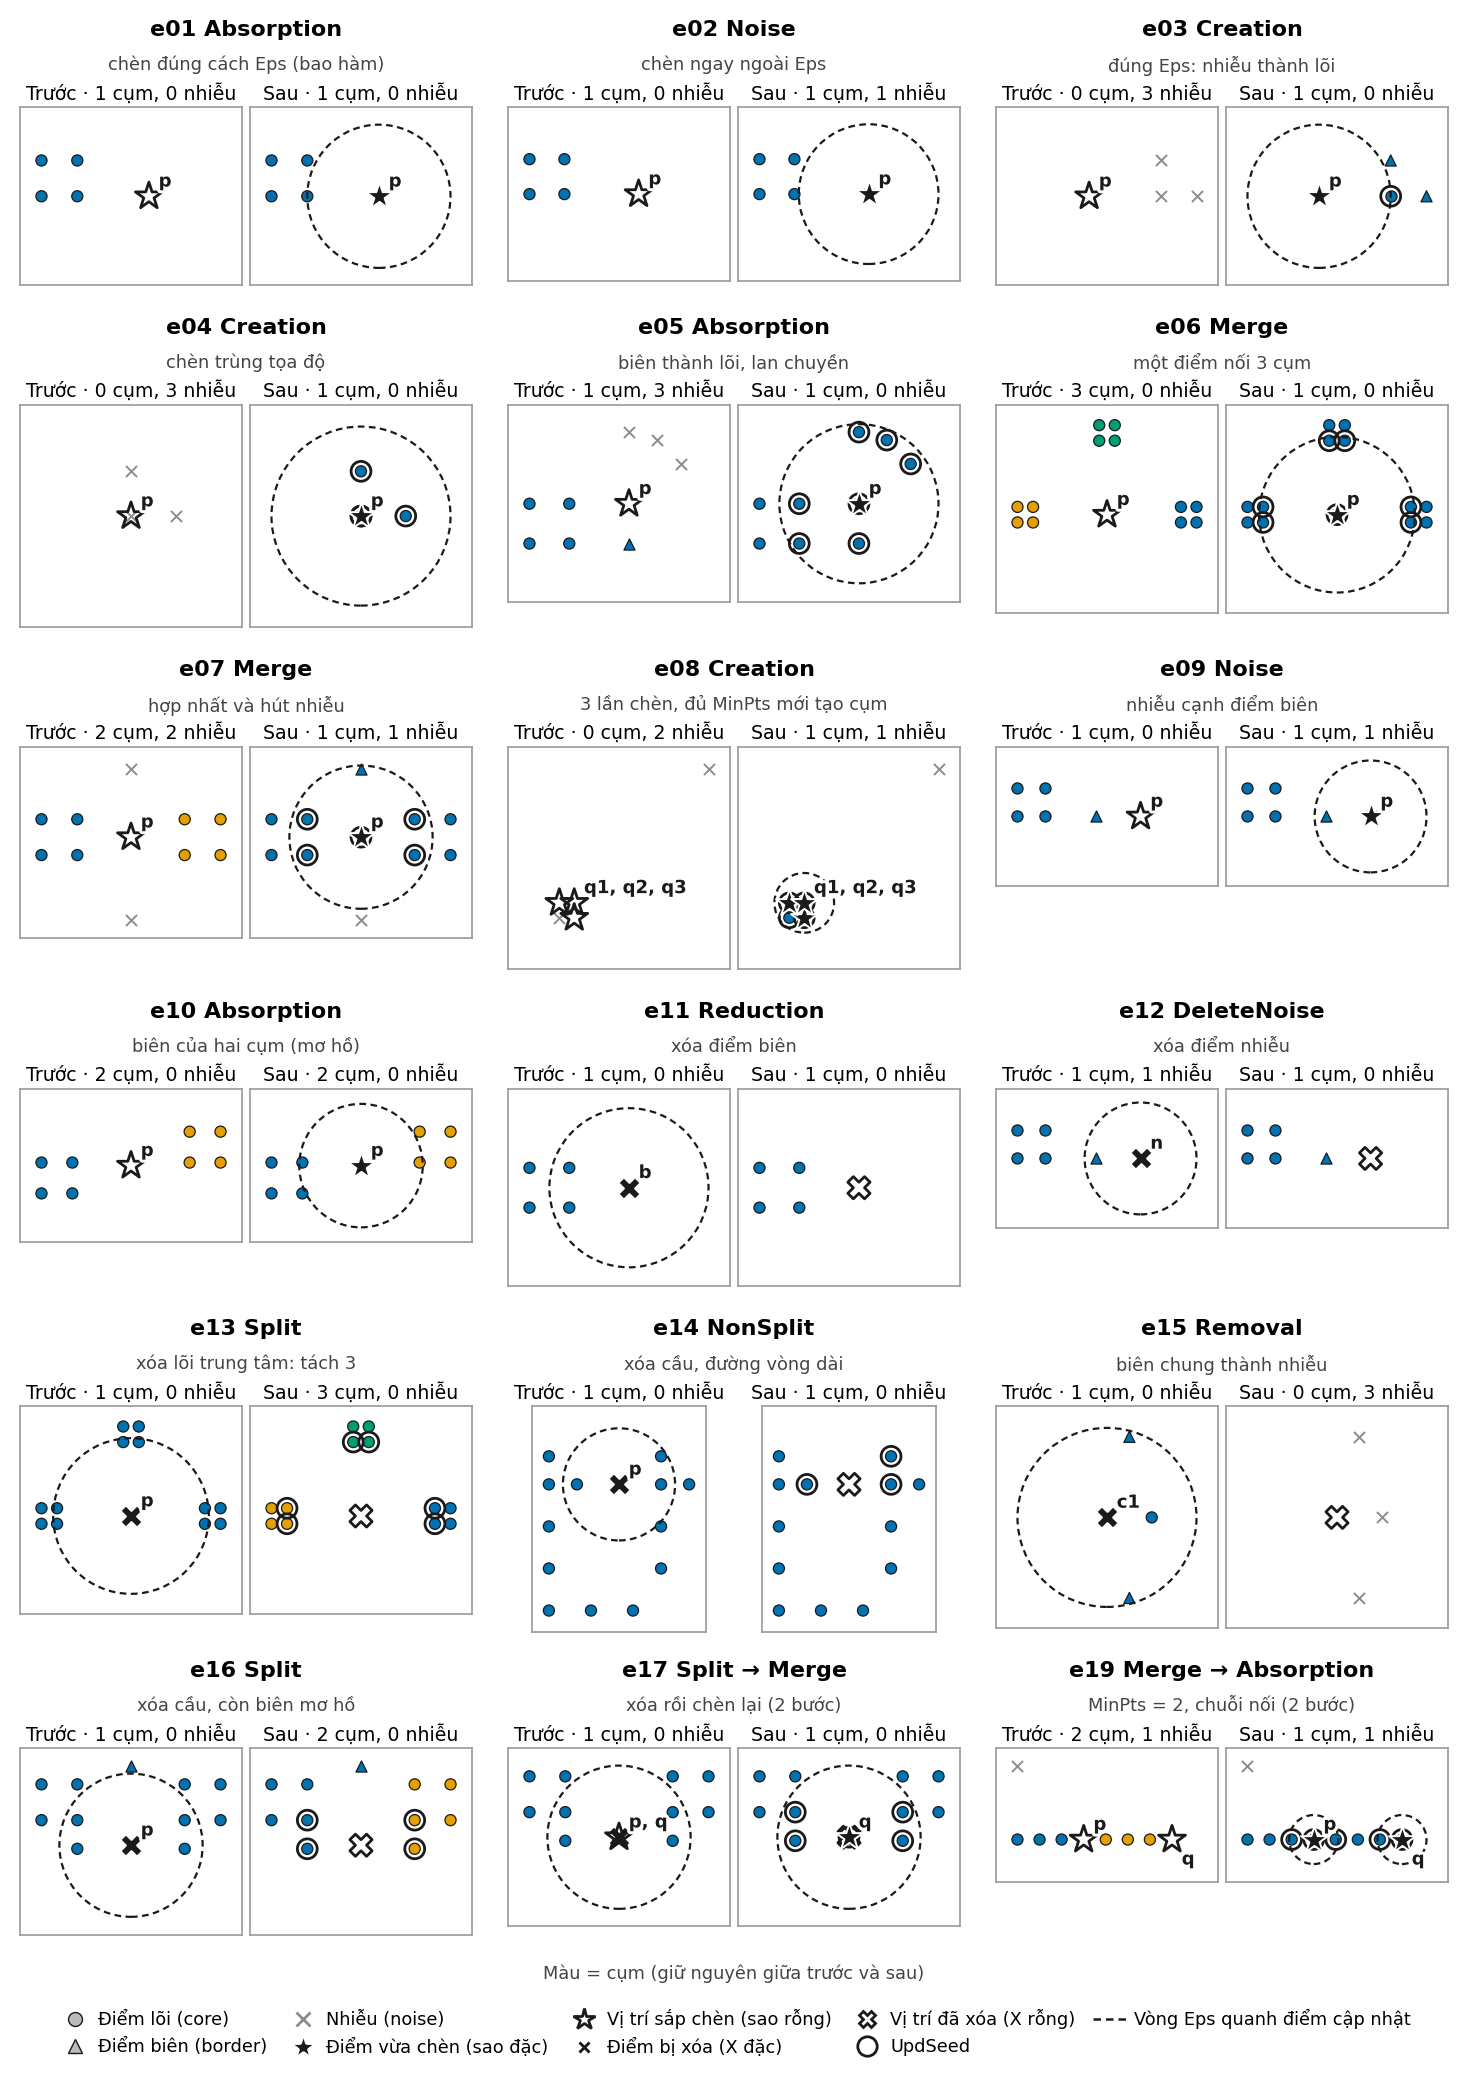
\includegraphics[width=\textwidth,height=0.72\textheight,keepaspectratio]{Images/case_gallery_edge.png}
\caption{Một số trường hợp biên bổ sung của thao tác thêm và xóa điểm}
\label{fig:appendix_edge_gallery}
\end{figure}

\begin{figure}[H]
\centering
    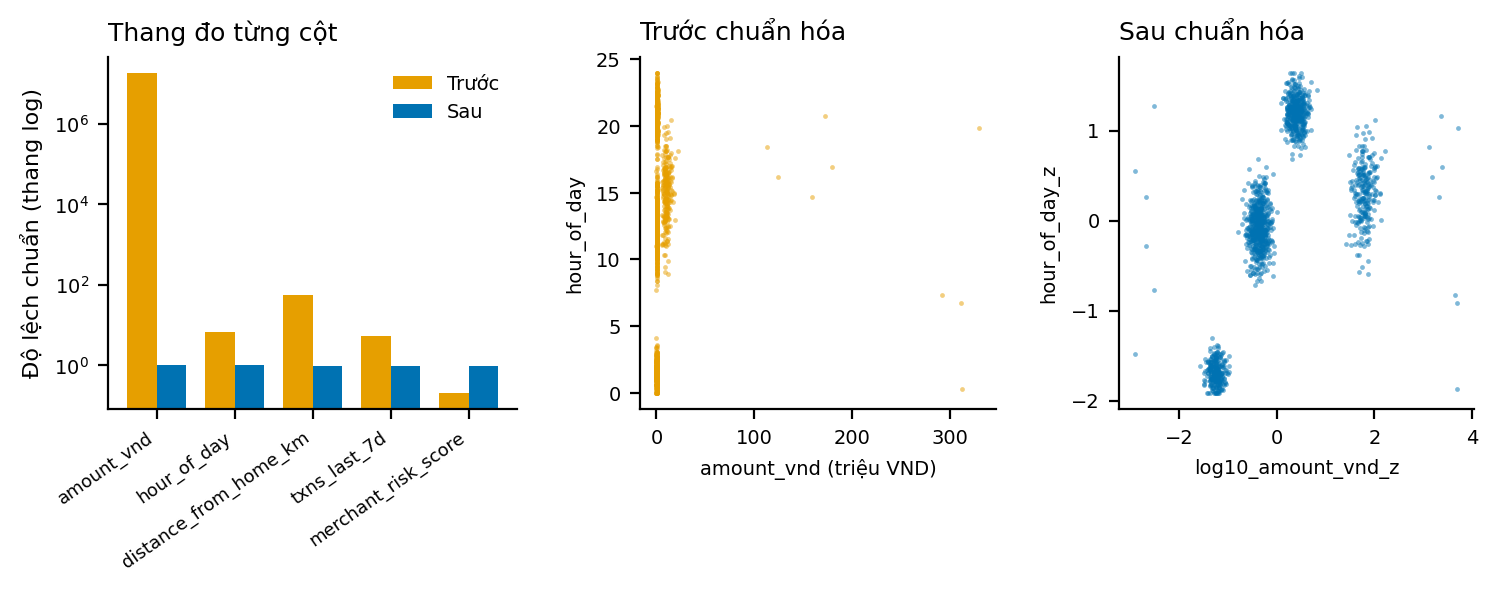
\includegraphics[width=\textwidth]{Images/scaling_effect_card.png}
\caption{Thang đo đặc trưng luồng thẻ trước và sau chuẩn hóa}
\label{fig:appendix_scaling}
\end{figure}
%
}{%
  \frontmatterchapter{PHỤ LỤC}%
}%
\end{document}
